\documentclass{ieeeaccess}
\usepackage{cite}
\usepackage{amsmath,amssymb,amsfonts}
%\usepackage{algorithmic}
\usepackage{graphicx}
\usepackage{textcomp}
\usepackage{algorithmicx}
\usepackage{algorithm}
\usepackage{algpseudocode}

\usepackage{lineno,hyperref}
\usepackage{booktabs}
\usepackage{tabularx}
\usepackage{longtable}
\usepackage{graphicx}

%\usepackage{subcaption}
\usepackage{caption}
\usepackage{mwe}
\usepackage{color}

\usepackage{graphviz}

\usepackage{booktabs}
\usepackage{multirow}

\newcommand{\myblue}[1]{\textcolor{blue}{#1}}
\newcommand\norm[1]{\left\lVert#1\right\rVert}

\usepackage[utf8]{inputenc}



\def\BibTeX{{\rm B\kern-.05em{\sc i\kern-.025em b}\kern-.08em
    T\kern-.1667em\lower.7ex\hbox{E}\kern-.125emX}}
\begin{document}
\history{Date of publication xxxx 00, 0000, date of current version xxxx 00, 0000.}
\doi{10.1109/ACCESS.2017.DOI}

\title{Forecasting Promotional Sales within the Neighbourhood}

\author{\uppercase{{Carlos}~Aguilar-Palacios}\authorrefmark{1},
\uppercase{Sergio~Mu\~noz-Romero}\authorrefmark{1,2},
\uppercase{and Jos\'e~Luis~Rojo-\'Alvarez}\authorrefmark{1,2}~\IEEEmembership{Senior~Member,~IEEE}}

\address[1]{Department of Signal Theory and Communications, Telematics and Computing Systems, Universidad Rey Juan Carlos, Madrid}
\address[2]{Center for Computational Simulation; Universidad Polit\'ecnica de Madrid, Madrid}

\tfootnote{This work was partly supported by Research Grants FINALE, and KERMES (TEC2016-75161-C2-1-R, and 
TEC2016-81900-REDT/AEI) from Spanish Government.}

\markboth
{Aguilar-Palacios~C. \headeretal: Preparation of Papers for IEEE TRANSACTIONS and JOURNALS}
{Aguilar-Palacios~C. \headeretal: Preparation of Papers for IEEE TRANSACTIONS and JOURNALS}

\corresp{Corresponding author: Carlos~Aguilar-Palacios (e-mail: carlos.aguilar.palacios@gmail.com).}

\begin{abstract}
Promotions are a widely used strategy to engage consumers and as such, retailers dedicate immense effort and resources to their planning and forecasting. This paper introduces a novel interpretable machine learning method specifically tailored to the automatic prediction of promotional sales in real-market applications. Particularly, we present a fully-automated weighted k-nearest neighbours where the distances are calculated based on a feature selection process that focuses on the similarity of promotional sales. The method learns online, thereby avoiding the model being retrained and redeployed. It is robust and able to infer the mechanisms leading to sales as demonstrated on detailed surrogate models. Also, to validate this method, real market data provided by a worldwide retailer have been used, covering numerous categories from three different countries and several types of stores. The algorithm is benchmarked against an ensemble of regression trees and the forecast provided by the retailer and it outperforms both on a merit figure composed, not only by the mean absolute error, but also by the error deviations used in retail business.
The proposed method significantly improves the accuracy of the forecast in many diverse categories and geographical locations, yielding significant and operative benefits for supply chains. Additionally, we briefly discuss in the Appendix how to deploy our method as a RESTful service in a production environment.
\end{abstract}

\begin{keywords}
Automated Feature Selection, weighted k-Nearest Neighbours, Online Learning, Predictive Models, Promotions, Supply Chain, Non-Negative Least Squares.
\end{keywords}

\titlepgskip=-15pt

\maketitle

\section{Introduction} \label{sect:Intro}

\PARstart{S}{ales} promotions are marketing strategies used by retailers to stimulate the demand of products. In addition to being profitable, promotions also help to reduce stockpiling, attract customers, build store traffic, introduce new products and counteract competitors \cite{gomez2007empirical, ailawadi2006promotion, natter2007practice}. Typically, retailers use a variety of approaches to promote products, including: price discounts, special deals (buy-one-get-one-free), vouchers, rebates and special displays \cite{blattberg1990sales}. Even when these factors are within the retailer's remit, there are external components that determine the performance of a promotion, including the following: macro-economic changes, competitors, sensitivity to market trends, sales in complementary and competitive categories and seasonal effects \cite{blattberg1995promotions}. From the perspective of the retailer, the estimation of promotional sales is pivotal in supporting inventory and production planning for supply chains \cite{fildes2016use}, operational decisions and also for reducing waste. For customers, accurate forecast results in adequately stocked shelves and an improved shopping experience. Manufacturers and suppliers also benefit from sharing forecast information~\cite{alamdar2018pricing}.

The promotional planning process is complex and challenging \cite{ma2017retail}, and it must account for changes in a dynamic and highly competitive market. As a result, retailers employ forecasters, who are dedicated analysts anticipating the future sales of products on offer. It is not uncommon for these teams to be divided into categories, such as "fresh" or "grocery", where the forecasters develop rules of thumb based on their experience and intuition to predict the sales. Due to the complexity and large number of promotions, many retailers have implemented forecasting decision support systems, casting these rules into heuristic algorithms that aid the forecasters. Some retailers have also applied statistical and machine learning approaches proposed by academia \cite{van2016analysis,di2016application,ramanathan2011identifying,ali2009sku}.
All of these methods rely on information from historical sales to forecast future sales. However, only a fraction of them are able to provide an interpretation behind the figures. This lack of a comprehensive explanation complicates business decisions. Even if methods such as Decision Trees, Neural Networks, or Support Vector Machines could provide more accurate predictions, forecasters and managers need to be convinced of the rationale behind the results, even if it means sacrificing accuracy for informativeness \cite{louis2013analysts}. %Of is better than 'Amongst' 
Amongst the methods that provide contextualisation, linear approaches are generally not accurate enough (see Experiment~\ref{subSect:muticol}). Whilst heuristic ones are, they are often difficult to adapt to new scenarios.

Ideally, a forecasting algorithm for promotions should be adaptable, interpretable, accurate, and stable. Adaptability requires that the algorithm performs well under distinct categories, different geographical locations and market changes, all factors which impact product sales. Stability requires that the accuracy does not dramatically depend on time, so the model does not need to be continually refreshed. This minimises the downtime required by re-training, testing and re-uploading, a significant issue for worldwide retailers.

In this paper we present a new method to forecast promotions founded on online learning k-nearest neighbours (kNN). The kNN algorithm is a well-known non-parametric method that has been successfully applied for decades to a multitude of problems and it still continues to be a topic of interest in predictive applications~\cite{LIU2011fast,CHEN2017feature,martinez2018dealing}. \myblue{Our variant of kNN searches for the closest promotions using a distance that is scaled by the relevance of each feature. Each stock keeping unit (SKU) is treated independently and the past promotions are used to train the algorithm. To produce a forecast, the inverse of these distances constitute the weights of a weighted average that aggregates the past sales. The method has been developed and tested on surrogate models and real market promotional data from a worldwide retailer, covering several categories (fresh food, grocery, beauty products and drinks) in 3 different countries with different types of stores. It is lightweight and interpretative and the results} can be easily modified by an operator in a cost-efficient framework, overcoming the classical view of a demand forecasting being costly~\cite{shin2010firms}.

The rest of the paper is organised as follows. First, Section~\ref{sect:Intro} illustrates promotions and their mechanisms. Section~\ref{sect:Promotions} contextualises promotions and presents the framework used in this paper. Section~\ref{sect:Model} describes the proposed method. Section~\ref{sect:Experiments} describes the experiments including data description and error metrics and presents the results on actual data and Section~\ref{sect:Conclusion} discusses the method and its suitability to support managers and forecasters in market environments.

A Python implementation of the method is available in \url{https://github.com/CarlitosDev/nextDoor/}.


%% ############################################
\section{Promotions} \label{sect:Promotions}

In this section, we introduce some key concepts about promotions and their mechanisms along with the framework and notation used in this paper. As previously stated, scientific literature on promotions based on machine learning algorithms is often applied mostly from a data matrix problem statement, without paying attention to the specific peculiarities of the problem. In this work we establish a general framework on our promotional scenario linking the data generation, statistical description of promotional processes, data sampling corresponding to different controlled and uncontrolled situations, and finally the corresponding matrix description of the problem.
Matrices are denoted as uppercase boldface letters whereas vectors are denoted as lowercase boldface letters. In our framework, promotion models rely on data sampled from multidimensional random processes that are usually given by a mix of quantitative and qualitative variables.

% Using 'plotAPromotion.m'
%\Figure[t!](topskip=0pt, botskip=0pt, midskip=0pt){figs/aguil1.png}
%{Product history covering 14 months in an Asian country. The upper chart shows the nationwide normalised sales, being the promotional periods the ones shadowed in gray colour whereas the normal sales are white coloured. The sales seem to have a weekly pattern and there are 3 clear peaks corresponding to the end of the year and a national festivity. The bottom chart shows the normalised price of the item during that 14 months period and it intends to illustrate that the relationship between price and sales is not direct.\label{fig:promotionsModel}}

% Using 'plotAPromotion.m'
\begin{figure*}[t]
  \centering 
  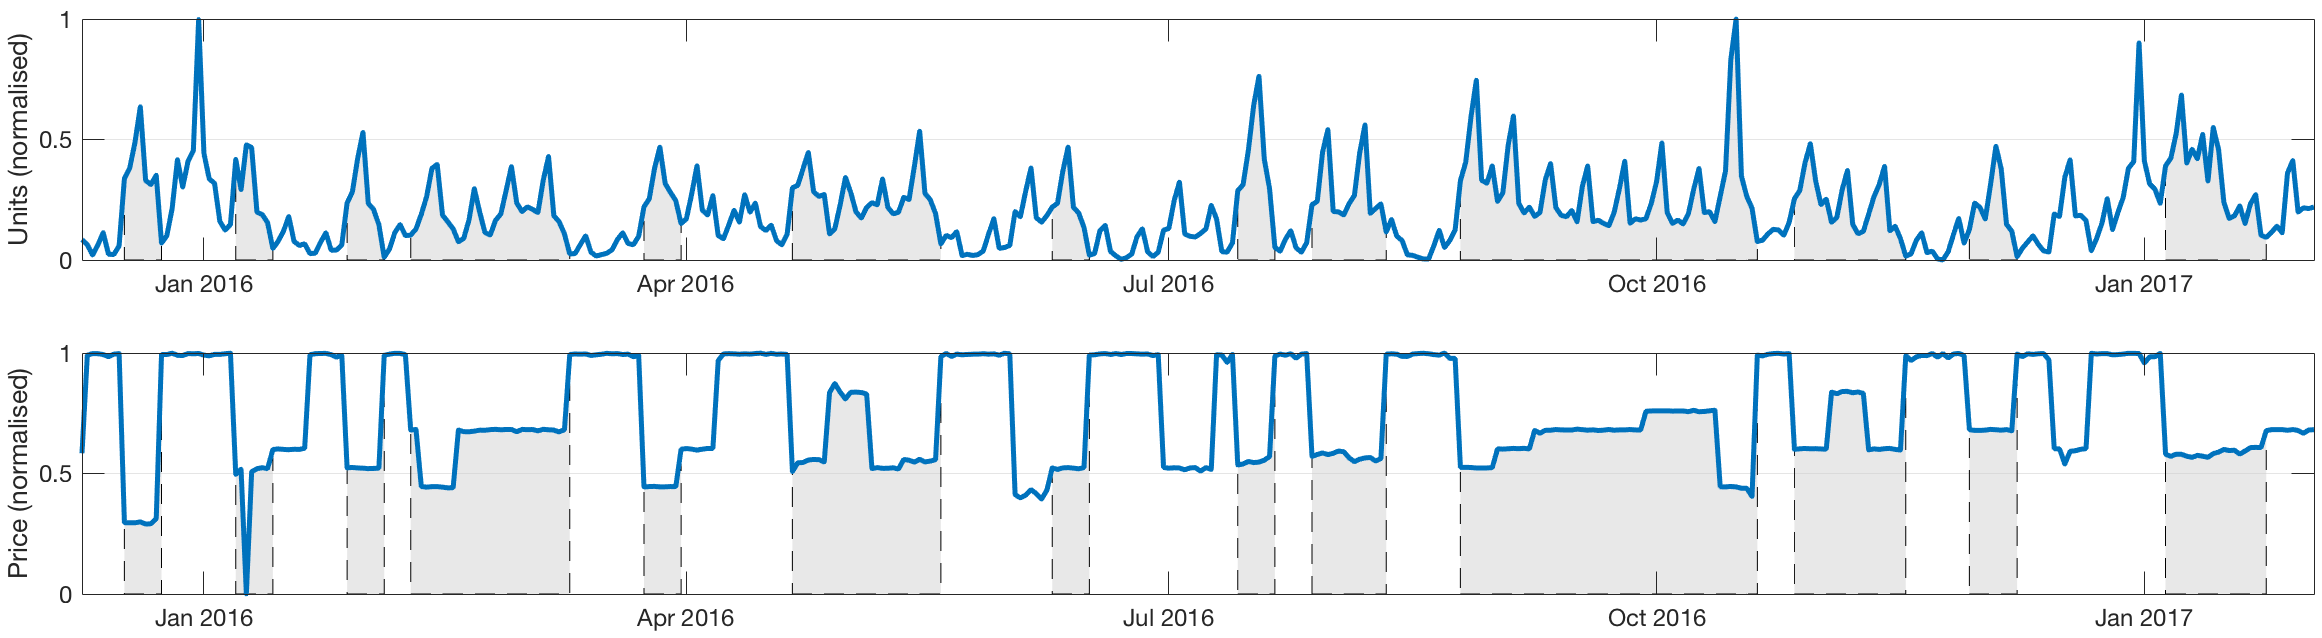
\includegraphics[width=\textwidth]{figs/aguil1.png} 
  \caption{Product history covering 14 months in an Asian country. The upper chart shows the nationwide normalised sales, being the promotional periods the ones shadowed in gray colour whereas the normal sales are white coloured. The sales seem to have a weekly pattern and there are 3 clear peaks corresponding to the end of the year and a national festivity. The bottom chart shows the normalised price of the item for the same period. This graph intends to illustrate that the relationship between price and sales is far from simple.}
  \label{fig:promotionsModel}
\end{figure*}

A promotion that is launched on a particular product can be seen as a collection of parameters that the retailer devises in order to attract customers, and ultimately to increase sales. As mentioned in Section \ref{sect:Intro}, the retailer controls certain factors and not others, e.g. competitors, economic climate, or trends. Amongst the controlled factors, one of the variables that influences sales the most is price. A common strategy amongst retailers is known as "price cut" pertaining to promotions, which is a direct reduction in the regular price of a given item. More forms of price reductions are in the likes of \textit{buy one (or more) and get one (or more) free}, where a minimum number of items is required to trigger the offer. The duration of the promotion is another relevant variable, ranging from offers lasting for one or two days, to the the usual biweekly or monthly cycles or to the more permanent ones known as \textit{rollbacks} that can last for months. Festivities, events and holidays are also important factors when running promotions. Some products are very seasonal, such as Christmas paraphernalia, whereas some products are sold all year long but tend to peak at particular times,  motivating campaigns such as \textit{back to school}. It is worth mentioning that some of these campaigns promote similar products resulting in a cannibalisation effect. Another aspect of promotions is that retailers might direct promotions to groups of stores, as opposed to nationwide offers, and also the SKU on offer might present different prices for different types of stores. Regarding time and dates, some products are heavily seasonal concentrating the sales in certain periods of the year. There are also products that tend to be purchased during particular days of the week, and for some countries payday is also important. Holiday and local festivities dramatically impact promotional sales. In terms of measuring the success of a promotion, a common key performance indicator (KPI) are the sales. For some retailers, it is given by the total amount of sold units, but more commonly it is a compound measure of the sales along with some market performance indicators. The sales performance of a promotion is holistic, as each feature plays a different role. A collection of descriptive features is pivotal in understanding it, otherwise, and as depicted by Figure \ref{fig:promotionsModel}, the information about item price is not enough to infer the unit sales.



%\subsection{Framework for promotions} \label{sect:framework}

Let us establish in this section our framework to operate with promotional information. Firstly, a promotion can be described as a paired biset $(\mathbf{x},y)$, where $y \in \mathbb{R}$ is the response variable or KPI, and $\mathbf{x}$ is a vector of the parameters that describe the promotion itself and determine the response variable to an extent, as there are other factors that are not known. It is important to note the temporal intrinsic relationship among these variables, in such a way that parameters in $\mathbf{x}$ are all known before the promotion starts, whereas the KPI is only known at the end of the promotional period. 
The parameters that define a promotion and referred here as features, and they contain information in %quantitative and qualitative forms.
different data formats.
The part of $\mathbf{x}$ that contains $n_1$ continuous or metric features  information are random real processes $\{x_1^m, \ldots , x_{n_1}^m \}$ where each $x_i^m \in \mathbb{R}$ follows a probability density function ({\it pdf}) denoted by $x_i^m \sim f_{x_i^m}(x_i^m)$. The % %qualitative 
non-metric counterpart are $n_2$ random categorical processes $\{x_1^c, \ldots , x_{n_2}^c \}$ where $x_i^c \in \mathcal{G}^{v_i}$ and $v_i$ is the number of possible values for $x_i^c$ within the set $\mathcal{G}$. Each $x_i^c$ follows a mass density function ({\it mdf}) $x_i^c \sim g_{x_i^c}(x_i^c)$. Therefore, $\mathbf{x} \in \mathbb{R}^{n_1} \times \mathcal{G}^{n_2}$ and it can be seen as a hybrid-type or heterogeneous multidimensional vector. Other types of features could be used as promotional information, which are not considered here, as for instance free-text documents, as far as they are not as usually available as the two preceding ones. 

In our framework, the data that we observe from historical promotions comes from the underlying joint distribution $p({\mathbf{x}}, y)$, which contains the description of the features and response variables as follows:

%\begin{eqnarray}
%p(\mathbf{x}) & = &\int_{<y>} p({\mathbf{x}}, y) \,dy  \label{eqn:aa1}
%\\ 
%p(y) & = & \int_{<\mathbf{x}>} p({\mathbf{x}}, y) \,d\mathbf{x} \label{eqn:aa2}
%\end{eqnarray}

\begin{IEEEeqnarray}{CCC}
\IEEEyesnumber\label{eq:both} \IEEEyessubnumber*
p(\mathbf{x}) & = &\int_{<y>} p({\mathbf{x}}, y)~dy  \label{eqn:aa1}
\\
p(y) & = & \int_{<\mathbf{x}>} p({\mathbf{x}}, y)~d\mathbf{x} \label{eqn:aa2}
\end{IEEEeqnarray}
where $< \cdot >$ denotes the corresponding integration domain. 
Our interpretation of $p({\mathbf{x}}, y)$ is that some of the variables contained in $\mathbf{x}$ (the available promotion context) determine to a great extent the value of $y$ (the actual promotion KPI). Therefore, our motivation is to be able to estimate the values of $y$ given the parameters in $\mathbf{x}$, which are known or even can be controlled when the promotion is planned. In probabilistic terms this corresponds to know the conditional or posterior probability of the KPI for a given value of the context, given by $p(y | \mathbf{x})$. In the case of having complete knowledge of the statistical distribution, we could use exact probabilistic data models to estimate the effect of the features vector on the response variable, as follows:
\begin{equation}
p(y | \mathbf{x}) = \frac{p(\mathbf{x} | y) p(y)} {p(\mathbf{x})}
\label{eqn:bayes}
\end{equation}

However, we do not hold the full knowledge of the distributions, instead we only have a limited number $N$ of sets of paired observations of these random processes, which can be formally expressed by:
\begin{equation}
p({\mathbf{x}}, y) \overset{S_u} {\longrightarrow} \{(\mathbf{x}_i, y_i), i=1, \ldots ,N\}
\label{eqn:uniform_sampling}
\end{equation}
where $S_u$ is an operator that generates $N$ samples uniformly distributed over the domains of $\mathbf{x}$ and $y$. This motivates us to use a parametric model whose  parameters are adjusted with the data available at the prediction time and in an online manner. Thus, we can estimate $y$ given $\mathbf{x}$ through the following equation:
\begin{equation}
y = \hat y + \varepsilon = \Gamma(\mathbf{x}) + \varepsilon
\label{eqn:ideal_estimator}
\end{equation}
where $\Gamma(\mathbf{x})$ is an ideal estimator of $y$ and $\varepsilon$ represents the unknown information that is not captured in the context $\mathbf{x}$ or retained by the estimating function $\Gamma$. To represent the full set of $N$ observed historical promotions, let us introduce the following matrix notation $\mathbf{X} = \left[\mathbf{x}_1,~\mathbf{x}_2,~\ldots,~\mathbf{x}_N \right]^\top$ and  $\mathbf{y} = \left[y_1,~y_2,~\ldots,~y_N \right]^\top$ so that set $\mathcal{D}$ is formed by concatenating as per $\mathbf{x}$ and $y$, i.e.,  $\mathcal{D} = \{(\mathbf{x}_1, y_1), ~\ldots , (\mathbf{x}_N, y_N)\}$, generally, $\mathcal{D} = \{\mathbf{X}, \mathbf{y}\}$. This is a usual notation in machine learning literature, and $\mathbf{X}$ is often called the input data matrix, or simply the data matrix.


Also, let us define an operator $\Psi$, in such a way that given a set of feature observations and a vector of free parameters $\boldsymbol{\theta}$ controlling its adjustment, it yields a function $g$ that approaches to the ideal estimator $\Gamma$, formally denoted as:
\begin{equation} 
g = \Psi(\mathbf{X}, \mathbf{y}, \boldsymbol{\theta)} \Rightarrow g(\mathbf{x}) \rightarrow \Gamma(\mathbf{x})
\label{eqn:aa5}
\end{equation}
Hence,  operator $\Psi$ is used to estimate the value of the response variable of a new promotion given the set of features $\mathbf{x}_p$ as follows:
\begin{equation}
\hat{y}_p = g(\mathbf{x}_p) + e_p
\label{eqn:aa6}
\end{equation}
Note that operator $\Psi$ and its free parameters $\boldsymbol{\theta}$ represent on a general view any machine learning estimation algorithm that can be built from a set of the observed and available promotional data. Therefore, this operator includes all the design stages that are usually necessary to ensure generalisation, this is, the strategy followed for splitting the available data set into a training and a test set. Function $g$ is usually a non-parametric expression, in the sense that operator $\Psi$ has an implicit stage for estimating some set of model weights according to the training and test subsets. If we denote by $\mathbf{w}$ the set of model weights that are intrinsically estimated by the algorithm, we can see that the intermediate stage can be expressed as follows:
\begin{equation}
\mathbf{w} = \Psi(\mathbf{X}, \mathbf{y}, \boldsymbol{\theta}) \Rightarrow   \hat y_p =  g(\mathbf{w},\boldsymbol{x}_p) 
\label{eqn:aa7}
\end{equation}
where we have made explicit that function $g$ depends also on the estimated model weights. Nevertheless, the compact representation in Eq.\eqref{eqn:aa5} is usually enough for our notation and estimation process description.


\begin{figure}
  \centering 
      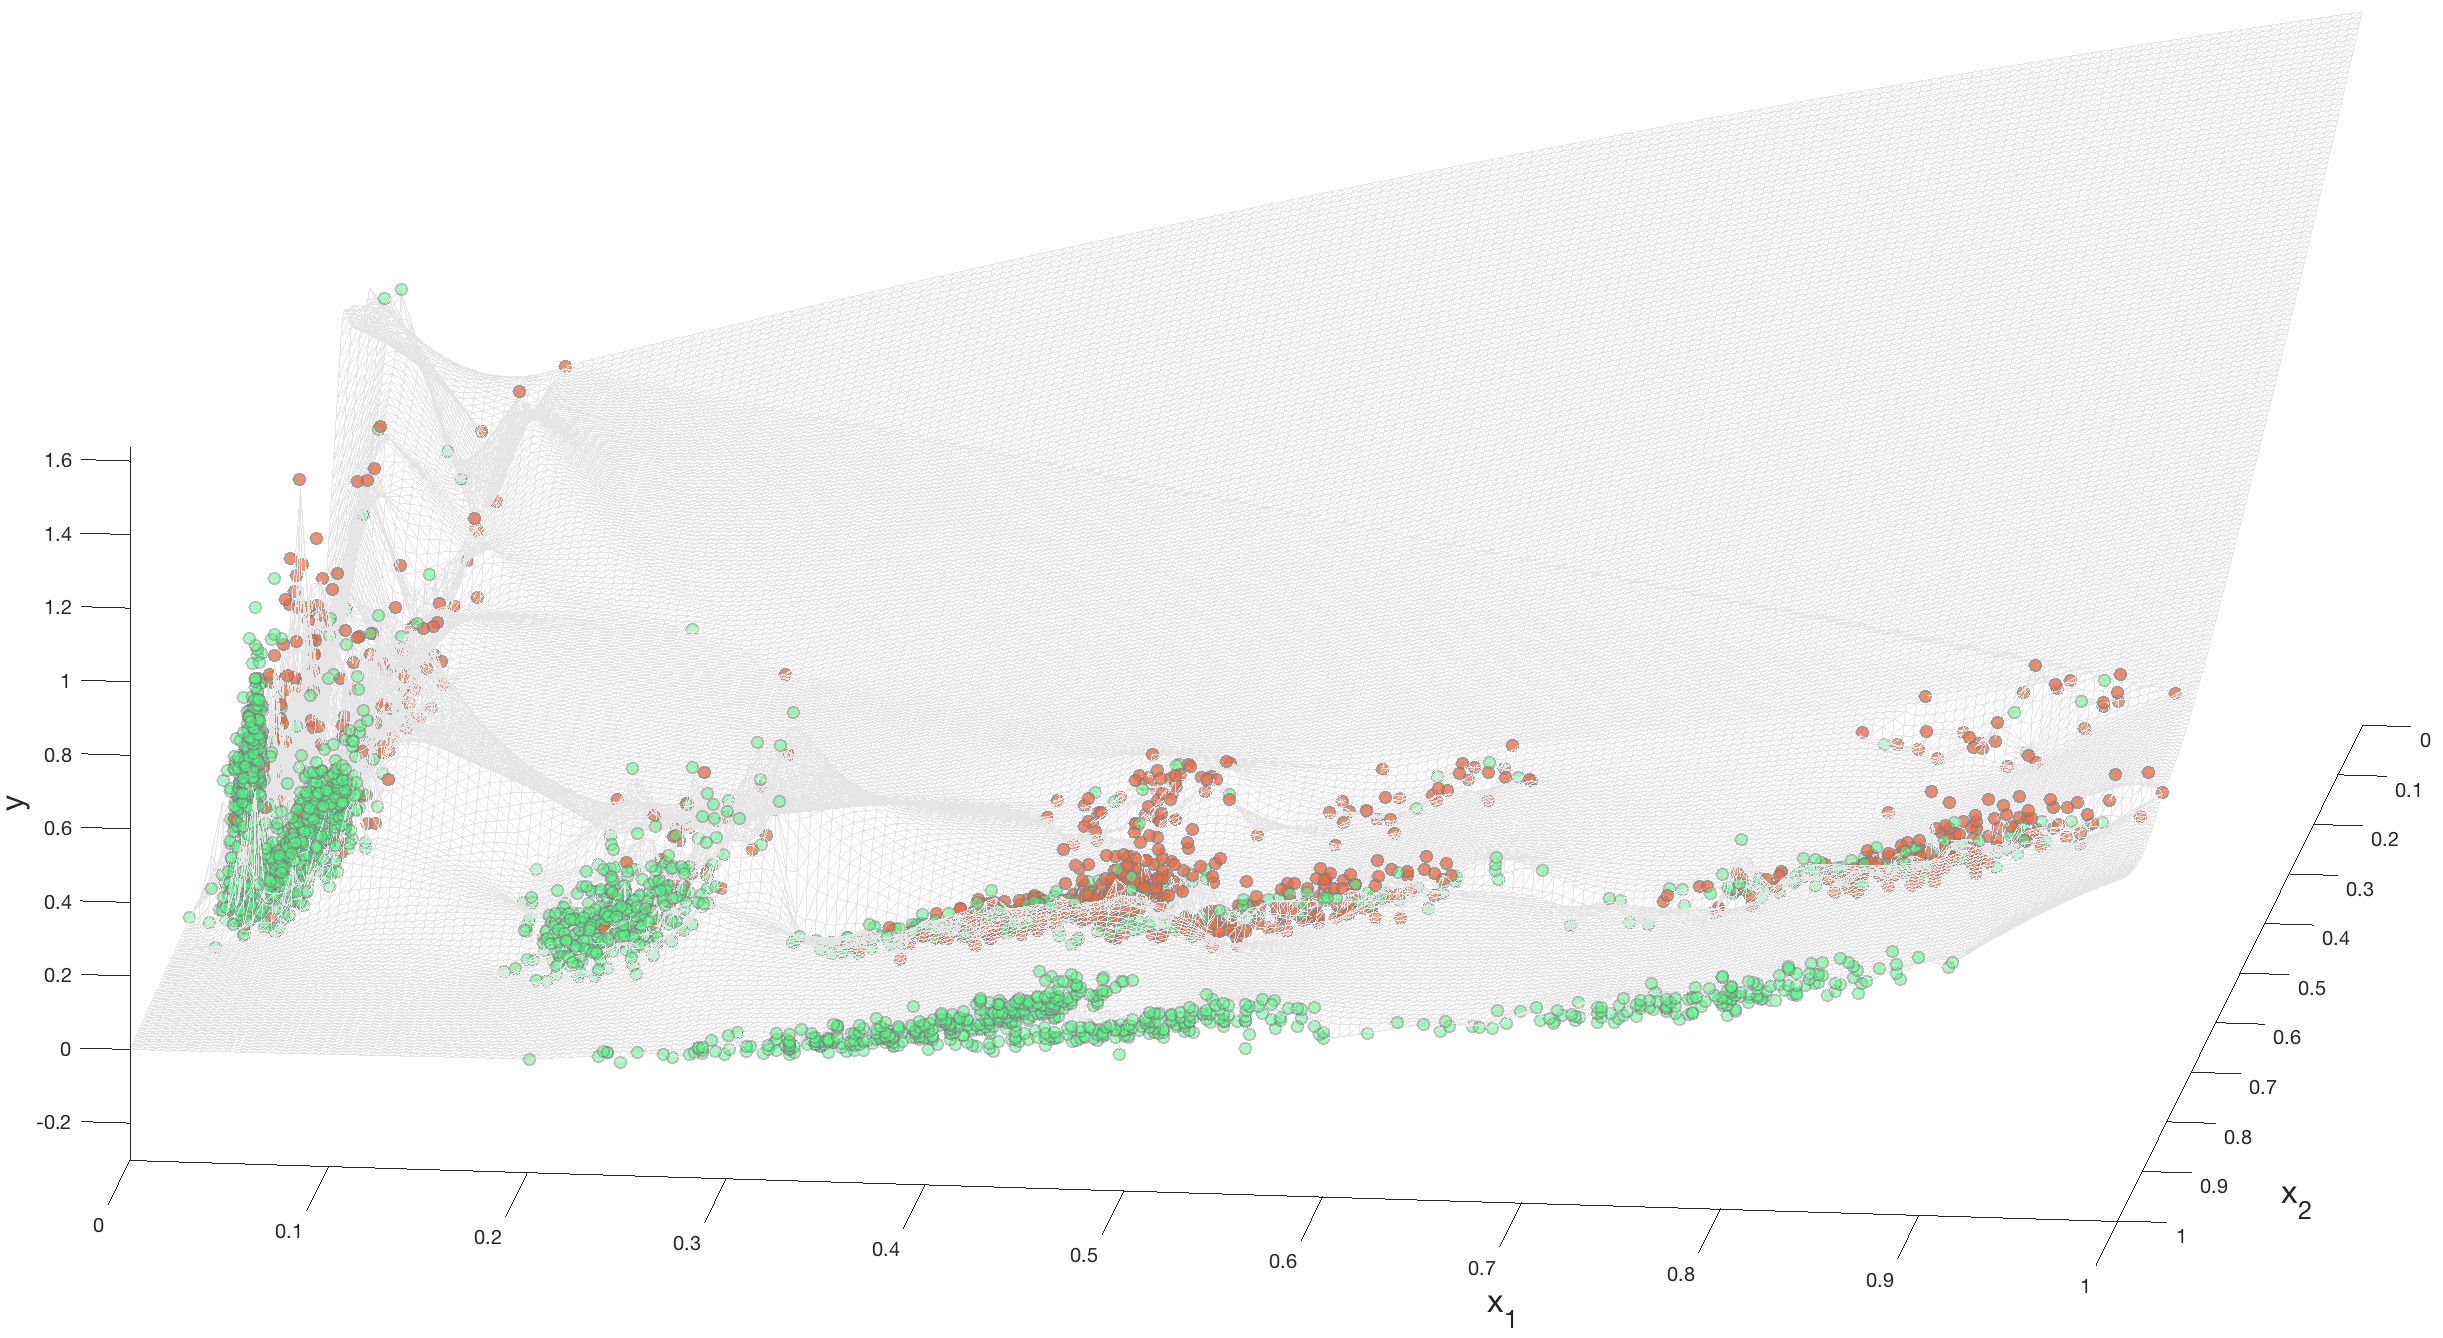
\includegraphics[width=\columnwidth]{figs/aguil2.png} 
  \caption{Promotional sales and regular sales are typically intertwined. This picture shows the normalised price and number of stores, axes $\mathbf{x_1}$ and $\mathbf{x_2}$ respectively, plotted against the normalised sales, distinguishing between regular sales in green colour and promotional sales in red.}
  \label{fig:promotionsSampling}
\end{figure}




The machine-learning based promotional modelling can be seen then as a nonlinear multidimensional regression problem. Figure \ref{fig:promotionsSampling} depicts, for visualisation purposes, a set of promotional sales as a function of two context variables. It can be clearly seen that these variables are not enough to account for a quality model of the promotion dynamics, and more explanatory features should be included to unfold the changes in KPI. Nevertheless, the grey surface represents the existence of a smooth surface accounting for the dynamics at this amount of explanatory features, which allows us to abstractly visualise what is happening when moving to higher dimensional input spaces.

%We only have a set of paired observations of these paired random processes, formally, 

%\begin{equation}
%p({\mathbf{x}}, y) \overset{S_u} {\longrightarrow} \{(\mathbf{x}_i, y_i), i=1, %\ldots ,N\}
%\label{eqn:aa3}
%\end{equation}

%where $S_u$ is an operator that generates $N$ samples uniformally distributed over the domains of $\mathbf{x}$ and $y$.

%Through statistical uniform sampling of this distribution, denoted as $S_u$, we form the set $\mathcal{D}$, given by

%\begin{equation}
%p({\mathbf{x}}, y) \overset{S_u} {\longrightarrow} \mathcal{D} = \{(\mathbf{x}_1, %y_1), \ldots , (\mathbf{x}_M, y_M)\}
%\label{eqn:eq_minus2}
%\end{equation}

%where $\mathcal{D}$ is the set of $M$ observed promotions that are available at the time of observation.


%We model the problem from the probabilistic perspective, a parametric model assuming that the expected prediction error is normally distributed (which we can experimentally verify).

% The kNN problem from a probabilistic perspective, assuming that the error in approximation resembles a gaussian distribution
%\begin{equation}
%p(\mathbf{y} | \mathbf{X}, \theta) = \mathcal{N}(\mathbf{y} | f(\mathbf{X}),\sigma^2(\mathbf{X}))
%\label{eqn:eq1}
%\end{equation}

%Being $\sigma^2(\mathbf{X})=\sigma^2$ and $f(\mathbf{X})$ the nearest neighbours approximation with parameters $\theta$ = (\mathbf{w}, \sigma^2)$.

Some specific problems can be stated from this model notation that are well-known in the statistical literature and are likely to be present in the promotional data. On the one hand, collinearity effects can be implicit in the data, which can be denoted as:
\begin{equation}
p({\mathbf{x}}, y) \overset{S_{cx}} {\longrightarrow} \{(\mathbf{x}_i, y_i), i=1, \ldots ,N\}
\label{eqn:collinear_sampling}
\end{equation}
The collinearity sampling operator $S_{cx}$ indicates that, rather than uniformly sampling in the $\boldsymbol{x}$ multidimensional space, input space is sampled through a constrained and often linear-like region, given by some linear sub-manifold of the space, with the average form:
\begin{equation}
\sum_{n=1}^{n_1} \beta_n x_n^m  = K
\end{equation}
where $K$ is a constant and some of the sub-manifold coefficients $\beta_n$ are different from zero. For those input features, not only the input domain is loose represented in the statistical sampling, but also those input features are highly correlated among them and secondarily with the output. Many estimation operators, such as the corresponding to least-square solution, exhibit problems to yield a stable solution at least in the available regions from the statistical sampling of the input space. 
This effect is present in many variables that can not be easily observed naturally throughout all their domain due to business constrains, for instance, existing promotional strategies can preclude from statistical sampling of some promotional combinations of strongly competing products. Collinearity is addressed in the experiments section~\ref{subSect:muticol}.

On the other hand, output subrepresentation can be also present on the data, which can be modelled as a different nonuniform sampling operator 
\begin{equation}
p({\mathbf{x}}, y) \overset{S_{sy}} {\longrightarrow} \{(\mathbf{x}_i, y_i), i=1, \ldots ,N\}
\label{eqn:nonuniform_sampling}
\end{equation}
This $S_{sy}$ sampling operator represents that a non-uniform sampling is performed in $y$ variable, which straightforwardly can be seen as inducing and unbalance of the represented promotions in the data. This is also due to the fact that historical promotions will be more likely driven by intuition and management principles, rather than trying to fulfil any criterion on statistical sampling. We address subrepresentation of promotions in the experiments section~\ref{subSect:MomsDay}.



% ##################################################
\section{Proposed Method for Modelling Promotions} \label{sect:Model}
%------------------------------------------------- %

\myblue{In this section we present our algorithm for the estimation of the promotional response to a set of known features, following the framework presented in Section \ref{sect:Promotions}.}

%%%%%%%%%%%
\myblue{Let us begin the section by describing the input data, the preprocessing step and the partition in training, validation and test sets. Typically the promotional data collected by retailers can be divided into four categories: numerical, binary, time-date variables and categorical. Amongst the numerical variables, is it common to find information about the number of stores running the promotion, the prices before the promotion is launched and during the promotion, as well as the discount.}

\myblue{Binary variables are used to inform about features such as a product being seasonal or the placement of a product on a featured display, amongst others.}

\myblue{Time and date information is converted to numerical or binary data in our model. For example, the starting date of a  promotion is decomposed into numerical variables representing the year, month, week of the month, day of the week and a numerical date. The duration of the promotion, as well as the number of days since the last promotion happened are are also stored. These variables are subsequently used in the preprocessing step to calculate the number of days and months between promotions and also to create binary flags indicating whether the promotions happen in the same year, month or week of the month, which are especially important for matching products that are seasonal or promotions that happen during festive periods.}

\myblue{Amongst the qualitative variables we typically find descriptors of the type of store or the type of promotion. As these variables present low cardinality, they have simply been converted to numerical data by using one-hot-encoding (OHE) transformation. In OHE, a categorical variable with $l_i$ labels is represented by $l_i$ binary predictors. Dimensionality-related issues for this input data codification are not expected to represent an issue in our datasets.}

\myblue{To create a model, the data for each individual product is divided into training, validation and test sets. These sets are chronologically organised and their sizes depend on the product itself. 
The training set contains the first M historical records, on average $74.99 \pm 65.57$ rows. It is followed by the validation test, which on average contains $18.74 \pm 16.13$ records. Finally, the test set is composed of the last promotion launched on all types of stores, averaging to $3.28 \pm 2.07$ records. Throughout the section the training set will be simply referred as $\mathbf{X}$.}

\myblue{After the preprocessing step, all the observed input features $\left[\mathbf{x}_1,\dots,\mathbf{x}_M\right]$ are of numerical type and therefore arranged into a matrix $\mathbf{X} \in \mathbb{R}^{M \times n}$. The observed promotion responses are grouped in vector $\mathbf{y} \in \mathbb{R}^{M}$. In the case of having missing values, which rarely occurs, we have opted to remove the record from the dataset.}


%have simply been converted to numerical by using one-hot-encoding (OHE) transformation, resulting in a total of $n=n_1+\sum_{i=1}^{n_2} v_i$ numerical predictors. We have used OHE as the variables that we will be using present low cardinality, so dimensionality related issues for this input data codification are not expected to represent an issue.

%%%%%%%%%%%

%As mentioned before, we group all the  observed input features $\left[\mathbf{x}_1,\dots,\mathbf{x}_M\right]$ into a numerical matrix $\mathbf{X} \in \mathbb{R}^{M \times n}$, where the qualitative variables have simply been converted to numerical by using one-hot-encoding (OHE) transformation, resulting in a total of $n=n_1+\sum_{i=1}^{n_2} v_i$ numerical predictors. We have used OHE as the variables that we will be using present low cardinality, so dimensionality related issues for this input data codification are not expected to represent an issue. All  the observed promotion responses are grouped in vector $\mathbf{y} \in \mathbb{R}^{M}$.

\myblue{One of the motivations of this paper is to estimate $y$ in an interpretative manner but also favouring direct modifications of the estimate. In this regard, the weighted arithmetic mean is a fairly simple manner of calculating the performance of a promotion at time $k$ based on the combination of $p \leq M$ historical realisations,} and this can be written as,

\begin{equation}
\hat{y}_k = \frac{\mathbf{w}^\top \mathbf{y}}{\mathbf{w}^\top \mathbf{1}}
\label{eqn:eqminus1}
\end{equation}

%One of the key concepts of our method is that in Eq.\eqref{eqn:eqminus1} $\mathbf{w}$ couples the historical observations of $\mathbf{y}$ and $\mathbf{X}$. These weights $\mathbf{w}=\left[w_1,\dots,w_p\right]^\top$ are calculated as $\mathbf{w} = \Psi(\mathbf{X}, \mathbf{y},  \boldsymbol{\theta})$ where $\Psi(\cdot)$ is a function that depends on the observed values of $\mathbf{X}$ and $\mathbf{y}$ and the vector of free parameters $\boldsymbol{\theta}$. Vector $\mathbf{1}$ is a column vector of all ones. Note that $\mathbf{w}$ are the weights mentioned in Eq.\eqref{eqn:aa7}.

A key concept of our method is that $\mathbf{w}$ couples the historical observations of $\mathbf{y}$ and $\mathbf{X}$. These weights $\mathbf{w}=\left[w_1,\dots,w_p\right]^\top$ are calculated as per Eq.\eqref{eqn:aa7} where $\Psi(\cdot)$ is a function that depends on the observed values of $\mathbf{X}$ and $\mathbf{y}$ and the vector of free parameters $\boldsymbol{\theta}$. Vector $\mathbf{1}$ is a column vector of all ones. For a forecaster, the prediction is easy to adjust by simply varying the contribution of the historical promotions.

% $\mathbf{w} = \Psi(\mathbf{X}, \mathbf{y},  \boldsymbol{\theta})$

The hypothesis behind $\Psi(\mathcal{D}, \boldsymbol{\theta})$ is that, for a given SKU, the promotions that sold a relatively similar number of units have something in common. In other words, very little time is needed with an expert forecaster to realise that, when being asked to predict the KPI of a promotion (or validate a forecast), firstly the forecaster will identify certain features that relate the promotion to forecast for and the historical ones, for example, similar price, number of stores or time of the year. With that idea of similarity, a prediction based on the past sales will be worked out. This expertise relies on selecting these features.

\myblue{To approximate the behaviour of the expert mathematically, $\Psi(\cdot)$ employs a matrix of distances $\mathbf{M}$ and vector of variable importance $\mathbf{v}$. %The matrix contains the differences between the features of promotions whereas the vector represents the importance of these features.
}

%-------------------------------------------------%
%\section{} \label{sect:Method}
%-------------------------------------------------%

%As indicated in the previous section, the method presented in this paper follows an online learning approach, consequently weights $\mathbf{w}$ must be derived from the available data $\mathcal{D}$ at the time of forecasting for each promotion.

%The function $\Psi(\cdot)$ that binds the KPI with the features does so through a matrix of distances and a vector of variable importance. In this step we aim to discover the relationship between the input features and the KPI on the training set, and use it to relate the new promotion to forecast for with the historical ones. 

%To find the impact of the input features in the promotional KPI, we repeat iteratively the following process. 
\myblue{Let us dive into the calculation of $\mathbf{M}$, which is a matrix indicating the differences between the features of promotions. From the training set $\mathcal{D}^{norm}$  where each feature has been normalised from 0 to 1, so $ 0 \leq x_{ij} \leq 1,  \forall x_{ij} \in \mathbf{X}$, we randomly extract a promotion $k$ with data $\{\mathbf{x}_k, y_k \} \subseteq \mathcal{D}^{norm}$.} The idea here is to quantify the closeness between the features of promotion $k$ and the remaining $M-1$ promotions in $\mathcal{D}^{norm}$, and to do that, first we define matrix $\mathbf{M}$ with the element-wise Euclidean distance as follows:
% $\mathbf{M} \in \mathbb{R}^{M-1 \times n}$
% use Sergio's notation
% X' is (m-1) x n
% 1 col vector is (m-1) x 1
% x_k is a row from X so 1 x n
\begin{equation} 
%\mathbf{M}^{(k)} = (\mathbf{X'}-\mathbf{x}^\top_k~\mathbf{1}^\top) \circ (\mathbf{X'}-\mathbf{x}^\top _k \mathbf{1}^\top)
\mathbf{M}^{(k)} = (\mathbf{X'}-\mathbf{1}~\mathbf{x}^k) \odot (\mathbf{X'}-\mathbf{1}~\mathbf{x}^k)
\label{eqn:featuresMatrix}
\end{equation}
%$$ \mathbf{M}^{(k)} = (\mathbf{X'}-\mathbf{x}^k~\mathbf{1}^\top) \circ (\mathbf{X'}-\mathbf{x}^k \mathbf{1}^\top)=
%\begin{bmatrix}
%    (x_{11}-x_{k1})^{2} & (x_{12}-x_{k2})^{2}  & \dots  & (x_{1n}-x_{kn})^{2} \\
%    \vdots & \vdots  & \ddots & \vdots \\
%    (x_{m1}-x_{k1})^{2} & (x_{m2}-x_{k2})^{2}  & \dots  & (x_{mn}-x_{kn})^{2}
%\label{featuresMatrix}
%\end{bmatrix},
%$$
% * <smunoz@tsc.uc3m.es> 2017-08-28T10:02:42.651Z:
% 
% Quizá estaría bien decir aquí que el superíndice (k) indica que los valores calculados se han hecho respecto a la promoción k-ésima. Algo así como: where superscript $(k)$ indicates that it has been calculated with respect to the $k$th promotion.
% 
% ^.
where superscript $(k)$ indicates that the result has been calculated with regard to the $k^{th}$ promotion. $\mathbf{X'} \in \mathbb{R}^{M-1 \times n}$ comes from matrix $\mathbf{X}$ where row $\mathbf{x}^k$ has been removed, and $\odot$ is the Hadamard product. Any measurement derived from matrix $\mathbf{M}$ implicitly assigns the same relevance to all of the features. As this is not the general case, we define a feature importance vector $\mathbf{v} \in \mathbb{R}_{+}^{n \times 1}$ that determines the importance of each variable by scaling the columns of $\mathbf{M}$. The closeness of each observation in $\mathbf{X'}$ to $\mathbf{x}^k$ is therefore the product $\mathbf{M}^{(k)} \mathbf{v}$. 

Based on $\mathbf{v}$ and $\mathbf{M}$, we can now define the weights $\mathbf{w}$ from Eq.\eqref{eqn:eqminus1} so the largest contributions come from the most similar promotions, as follows,
%
\begin{equation}
%w_i^{(k)} = \frac{1}{\sqrt{\mathbf{m}^i \mathbf{v}}} = \frac{1}{\sqrt{\sum_{j=1}^{n} v_j m_{ij}}}, ~~ i=1,\cdots,p.
w_i^{(k)} = \frac{1}{\sqrt{\mathbf{m}^i \mathbf{v}}} , ~~ i=1,\cdots,p.
\label{eqn:eq2}
\end{equation}
%
where $w_i^{(k)}$ is the contribution of historical promotion $i$ to forecast promotion $k$ and $\mathbf{m}^i$ is the $i^{th}$ row of matrix $\mathbf{M}^{(k)}$. By substituting Eq.\eqref{eqn:eq2} in Eq.\eqref{eqn:eqminus1}, we can formulate the problem of finding $\mathbf{v}$ can be tackled as minimising the norm forecast error,
%
\begin{equation}
\hat{\mathbf{v}}= \underset{\mathbf{v}*}{\arg\min} \left\{ \left\Vert y_k - \frac{ \sum_{i=1}^{p} \frac{1}{\sqrt{\mathbf{m}^i \mathbf{v}}} y_i} {\sum_{i=1}^{p} \frac{1}{\sqrt{\mathbf{m}^i \mathbf{v}}}}  \right\Vert^2 \right\}
\label{eqn:eq3}
\end{equation}
%\begin{equation}
%\hat{\mathbf{v}}= \underset{\mathbf{v}*}{\arg\min} \left\{ \left\Vert y_k - \frac{ \sum_{i=1}^{p} \frac{1}{\sqrt{\mathbf{m}^i \mathbf{v}}} y_i} {\sum_{i=1}^{p} %\frac{1}{\sqrt{\mathbf{m}^i \mathbf{v}}}}  \right\Vert^2 \right\} = \underset{\mathbf{v}*}{\arg\min} \left\{ \left\Vert y_k - \frac{ \sum_{i=1}^{p} %\frac{1}{\sqrt{\sum_{j=1}^{n} v_j M_{ij}}} y_i} {\sum_{i=1}^{p} \frac{1}{\sqrt{\sum_{j=1}^{n} v_j M_{ij}}}}  \right\Vert^2 \right\}
%\label{eqn:eq3}
%\end{equation}
which can be approached as an optimisation problem, although there are some issues around it for this particular application. Firstly, there is no guarantee that the chosen optimisation algorithm will always converge, and secondly, the computational burden results in large waiting times for the forecasters. Because of these issues, we propose a non-optimal approach based on the intuition that similar sales are driven by similar features. To illustrate our approach, let us define a set with two historical promotions $\mathcal{D}^{norm} = \{(\mathbf{x}_i, y_i), (\mathbf{x}_k, y_k)\}$. Our goal is to approximate the value of $y_k$ with just one observation, so the first step consists of setting the weight $w_i$ to a measure derived from the difference in sales,
\begin{equation}
w_i^{(k)} = \frac{1}{|y_k - y_i|}
\label{eqn:eq4}
\end{equation}
%
Substituting the definitions given for $w_i$ in Equations~\eqref{eqn:eq2} and \eqref{eqn:eq4} yields to:
\begin{equation}
%|y_k - y_i|^2 = \mathbf{m}^i \mathbf{v} = \sum_{j=1}^{n} v_j M_{ij}
|y_k - y_i|^2 = \mathbf{m}^i \mathbf{v}
\label{eqn:eq5}
\end{equation}
%
As the elements of vector $\mathbf{v}$ are positive real numbers, we can solve a non-negative least squares (NNLS) problem established as follows:
% Equation 7
\begin{equation}
\begin{aligned}
\hat{\mathbf{v}} =~ & \underset{\mathbf{v*}}{\arg\min}
& \{ \norm{ \mathbf{m}^i \mathbf{v} - e }_2
& + \lambda^2 \norm{ \mathbf{v} }_2 \}
&~~ \text{subject to}
&~\mathbf{v} \geq \mathbf{0}
\end{aligned}
\label{eqn:nnls}
\end{equation}
where $e=|y_k - y_i|^2$, and $\mathbf{v} \xrightarrow[e \to 0]{} 0$ and $\mathbf{v} \xrightarrow[e \to \infty]{} \infty$, meaning that  we assign a larger weight $w_i$ to a promotion that performed similarly than to a promotion that did differently.\footnote{Our KPI are measured in integer units (scaled when necessary). To grant numerical stability in Eq.\eqref{eqn:eq4}, the denominator is modified to $max\{1, |y_k - y_i|\}.$} The parameter $\lambda$ controls the amount of regularisation that prevents a variable to massively dominate the NNLS solution.

%promotion $k$ with the remaining $M-1$ promotions, 
To extend this formulation to the real case where the training set consists of $M$ observations, we define the differences vector $\mathbf{e}^{(k)} = [ |y_k - y_1|^2, \ldots , |y_k - y_{M-1}|^2 ]^\top$ and rewrite Eq.\eqref{eqn:eq5} in matrix form,
\begin{equation}
\mathbf{e}^{(k)}= \mathbf{M}^{(k)} \mathbf{v}^{(k)} \\
\label{eqn:eq6}
\end{equation}
%
%\subsection{Feature selection and sparsity}
And as described earlier, solve the problem with NNLS as:
% Equation 7
\begin{equation}
\begin{aligned}
\hat{\mathbf{v}} =~ & \underset{\mathbf{v*}}{\arg\min}
& \{ \norm{ \mathbf{M} \mathbf{v} - \mathbf{e} }_2
& + \lambda^2 \norm{ \mathbf{v} }_2 \}
&~~ \text{subject to}
&~\mathbf{v} \geq \mathbf{0}
\end{aligned}
\label{eqn:nnlsMatrix}
\end{equation}
%

We have established a framework to find the most relevant variables related to the sales of a promotion $k$. However, it is obvious that just one promotion does not represent the relationship between the features and promotional sales for a product. To gain wider insight into the features and also, to improve stability and accuracy, we repeat this process using a bootstrap aggregating (bagging) approach. In this step we repeat $B$ times  the process described above and average the results to obtain the feature importance vector $\mathbf{v}$, as outlined in Algorithm \ref{alg:1}.

%%%%%%%%%%%%% From Sergio: Pseudocódigo 1 %%%%%%%%%%%%%

\renewcommand{\algorithmiccomment}[1]{// #1}
\begin{algorithm}
%\setstretch{1.35}
%\addtolength{\belowcaptionskip}{6pt}
\caption{Pseudo-code for Feature Selection: Bagging}
\label{alg:1}
\textbf{Input:} $\mathbf{X} \in \mathbb{R}^{m\times n}$, $\mathbf{y} \in \mathbb{R}^{m\times 1}$, $B$, $C$, $P$, $t$ (consistency threshold).\\
\textbf{Output:} $S$: Set of relevant features. $\mathbf{v}$: Importance of the relevant features.\\
\begin{algorithmic}[1] 
\State With complete $\mathbf{X}$, normalise each variable.
\For{$b = 1 \to B$}
\State Retrieve the vector of predictors $\mathbf{x}^b$ from $\mathbf{X}$ and the sales $y^b$ from $\mathbf{y}$.
\For{$c = 1 \to C$}
\State Generate $\mathbf{X'}$ by sampling uniformly with replacement $P$ rows from $\mathbf{X}$ (excluding $\mathbf{x}^b$). The same applies to sales vector $\mathbf{y'}$.
\State With $\mathbf{X'}$ and $\mathbf{x}^b$, calculate the matrix of feature distances $\mathbf{M}^{(k)}$ using the definition from Eq.\eqref{eqn:featuresMatrix}.
\State Using $y^b$ and $\mathbf{y'}$, calculate the sales-based weights $\mathbf{w}$ as defined in Eq.\eqref{eqn:eq4}.
\State Find the variable importance vector $\mathbf{l}^c$ (being $\mathbf{l}^c$ the $c^{th}$ row of pool matrix $\mathbf{L} \in \mathbb{R}^{C\times n}$) using NNLS as per Eq.\eqref{eqn:nnlsMatrix}.
\EndFor
\State Set $\mathbf{a}^b$ = mean($\mathbf{L}$) where  $\mathbf{a}^b$ the $b^{th}$ row of pool matrix $\mathbf{A} \in \mathbb{R}^{B\times n}$.
\EndFor

\State Aggregate $\mathbf{A}$ throughout the $B$ iterations to obtain $\mathbf{f} = agg(\mathbf{A})$.
\For{$i=1 \to n$}
\If{$(\mathbf f)_i > t$} 
\State $S = S \cup (\mathbf x)_ i$
\State $\mathbf{v} = \mathbf{v} \cup (\mathbf b)_ i$
 \EndIf
\EndFor
\end{algorithmic}
\end{algorithm}

%- - - - - - - - - - - - - - - - - - %
%\subsection{The forecast}
Once we have the feature importance vector $\mathbf{v}$, forecasting a new upcoming promotion $k+1$ is a matter of two steps. First, matrix $\mathbf{M}^{(k+1)}$ is built using Eq.\eqref{eqn:featuresMatrix} to represent the feature distances between $k+1$ and the $M$ observations from the training set. The second step is to calculate weights $\mathbf{w}$ that scale the historical KPIs by combining $\mathbf{M}^{(k+1)}$ and $\mathbf{v}$ as follows,
\begin{equation}
\mathbf{w}^{(k+1)} = (\mathbf{M}^{(k+1)} \mathbf{v})^{-1/2}
\label{eqn:eq8}
\end{equation}
where $\mathbf{w} \in \mathbb{R}_{+}^{M}$. As mentioned in Section \ref{sect:Intro}, one of the motivations pursued in our algorithm is to be able to explain how the forecast is produced and also to be easily modified. The frequency of products going on promotion is very variable and it is not uncommon to find products in the training set that have been on special for at least 60 times in the last two years. The idea here is that, instead of presenting a forecast involving $M$ promotions in the training set, we select a representative subset of them, the so-called neighbours.

\begin{figure}
\centering
    %\includegraphics[width=\columnwidth]{figs/tikzoutput-figure0.pdf} 
    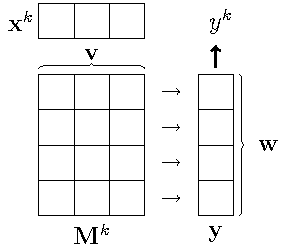
\includegraphics{figs/aguil3.pdf} 
    \caption{Diagram illustrating the forecasting process. For a new promotion $\mathbf{x}^{k}$, we first use the historical data to calculate feature weights $\mathbf{v}$. Then, distances matrix $\mathbf{M}^k$ is calculated using $\mathbf{x}^{k}$ and the historical data, where the columns are scaled by $\mathbf{v}$. With that information, we then calculate weights $\mathbf{w}$ that scale the historical values of the response variable $\mathbf{y}$ to produce the forecast $y^k$.}
\label{fig:graphicalWV}
\end{figure}

\myblue{The number of past promotions considered can be determined following different approaches. Based on our experiments, the best forecasting results are achieved when we cross-validate this number of neighbours on the validation set. To do this, for each promotion $(\mathbf{x}_p, y_p)$ in the validation set, we apply Eq.\eqref{eqn:eq8} sweeping the number of neighbours $k$ from 2 to the maximum number of historical promotions available, limited to a maximum of 15. Then we calculate the forecast error in each iteration and select the number of neighbours as the one that yields the minimum forecast error, as follows,}

\begin{equation}
k^{(p)} = \underset{k*}{\arg\min} \left\{ \left | y_p - \frac{ \sum_{i=1}^{k} w_i y_i} {\sum_{i=1}^{k} w_i}  \right | \cdot \frac{1}{y_p} \right\}
\label{eqn:eq_kNN}
\end{equation}

\myblue{The global number of neighbours is then determined by the average across all the validation set of the individual neighbours, formally $k = mean([k^{(1)}, \ldots, k^{(P)}])$. }The forecasting process is summarised in Figure~\ref{fig:graphicalWV}.


There are several technical considerations which are taken into account. Firstly, during the testing phase, we realised that bagging, despite its robustness, can take a longer training time than expected for an interactive application. So we looked for a faster alternative without significantly decreasing accuracy. We found a sub-sampling strategy that yields similar results in a fraction of the bagging time, summarised in Algorithm \ref{alg:2}. A comparison between both approaches is addressed in Section \ref{subSect:MomsDay}. Secondly, to improve the selection of features, the output of each expert can be combined to get a consensus of the most prominent variables. It also eases the set up of the hyperparameters as the idea behind ensemble learning is to combine experts with different features. And finally, at the cost of losing some interpretability, the method presented in this paper can be boosted to a strong forecaster. By selecting different training hyperparameters, we can create a set of weak forecasters and combine the predictions. This alternative to ensemble learning is tested in the experiments section and even if the results are positive, we do not recommend applying this approach as it sacrifices interpretability.

\renewcommand{\algorithmiccomment}[2]{// #2}
\begin{algorithm}
%\setstretch{1.35}
%\addtolength{\belowcaptionskip}{6pt}
\caption{Pseudo-code for fast Feature Selection: Sub-sampling}
\label{alg:2}
\textbf{Input:} $\mathbf{X} \in \mathbb{R}^{m\times n}$, $\mathbf{y} \in \mathbb{R}^{m\times 1}$, $B$, $P$, $t$ (consistency threshold).\\
\textbf{Output: } $S$: Set of relevant features. $\mathbf{v}$: Importance of the relevant features.\\

\begin{algorithmic}[2] 
\State With the complete $\mathbf{X}$, normalise each variable.
\For{$b = 1 \to B$}
\State Generate $\mathbf{X'}$ by sampling $P$ rows without replacement from $\mathbf{X}$, and the sales $\mathbf{y'}$ from $\mathbf{y}$.
\State Set the first row of $\mathbf{X'}$ as $\mathbf{x}^b$. Do the same for $y^b$.
\State With $\mathbf{X'}$ and $\mathbf{x}^b$, calculate the matrix of feature distances $\mathbf{M}^{(k)}$ using the definition from Eq.\eqref{eqn:featuresMatrix}.
\State Using $y^b$ and $\mathbf{y'}$, calculate the sales-based weights $\mathbf{w}$ as defined in Eq.\eqref{eqn:eq4}.

\State As per described in Eq.\eqref{eqn:nnlsMatrix}, find the variable importance vector $\mathbf{a}^b$ where $\mathbf{a}^b$ the $b^{th}$ row of pool matrix $\mathbf{A} \in \mathbb{R}^{B\times n}$.
\EndFor
\State Aggregate $\mathbf{A}$ throughout the $B$ iterations to obtain $\mathbf{f} = agg(\mathbf{A})$.
\For{$i=1 \to n$}
\If{$(\mathbf f)_i > t$} 
\State $S = S \cup (\mathbf x)_ i$
\State $\mathbf{v} = \mathbf{v} \cup (\mathbf b)_ i$
 \EndIf
\EndFor
\end{algorithmic}
\end{algorithm}

%-------------------------------------------------%
\section{Experiments and Results} \label{sect:Experiments}
%-------------------------------------------------%

After presenting the foundations of the method, this section details the validation through a series of four experiments. The first experiment addresses both collinearity and endogeneity as retailing data commonly suffer from these two issues, which can be problematic for various methods. The second experiment feature selection in a typical business scenario such as promotional events. To evaluate the selection of pivotal variables, a simulated surrogate model that mimics Mother's Day was built, and the positive results prove the feature selection capabilities. The third experiment deals with hyper-parameter tuning on a real dataset consisting on 361 sales promotions for a European country concluding with a set of recommended parameters. The fourth experiment evaluates the algorithm on a large real-market dataset consisting on thousands of promotions from three different countries and types of stores.

\myblue{In the following experiments, we benchmark our method against Least Squares (LS), an ensemble of regression trees and the retailer's forecast, where available. We have deliberately not included methods that are not directly interpretable, such as, SVM-r or widely used deep learning architectures such as Long Short-Term Memory (LSTM) or Gated Recurrent Units (GRUs).}

%- - - - - - - - - - - - - - - - - - %
\subsection{Collinearity and Endogeneity} \label{subSect:muticol}

In this experiment we address the performance of our method under collinearity and endogeneity conditions. Collinearity is a phenomenon in which one of the predictors is linearly related to another predictor. Commonly, promotional data presents linearly related variables, for example price and discount. Endogeneity refers to situations where the prediction error is correlated with one of the regressors. As mentioned in Section \ref{sect:Promotions}, not all the variables that impact the performance of a promotion can always be measured. To illustrate this situation, consider a variable $z$ that represents the affluence of shoppers in stores. It clearly impacts the sales $y$ but in this scenario it is not directly measured by the retailer. On the other hand, within the information that the retailer is able to collect from each promotion, there is a variable that measures the number of times a day the items in the shelves are restocked. In this scenario, $z$ affects both the independent and the response variable, and it is known as a confounding factor. Note the confounding variable corresponds to the $\varepsilon$ mentioned in Eq.\eqref{eqn:ideal_estimator}. A deeper explanation about endogeneity in Marketing Decisions Models can be found in~\cite{Shugan2004end}.

To assess the performance of our method under collinearity and endogeneity conditions, we forecast a controlled response variable where the generation mechanism (true model) is known, and it contains a bundle of independent, dependent and a confounding variable. For reference, we compare the model to the well-known and widely used LS one.

The experiment is divided into three different blocks. The first one, consists of applying our method (and LS) to an ideal scenario where all the information that contributes to the response variable is measured. The second block aims to evaluate the performance of our method under collinearity effects and compare it to the LS model. The third block demonstrates the performance of our method under endogeneity conditions and compare it again to the LS model.

The data model used in this experiment aims to reflect the sales distribution of an actual promotional product, a popular ready-to-eat vegetables box whose sales distribution is shown in Figure~\ref{fig:fakeProduct}.

\begin{figure}[t]
      \centering
      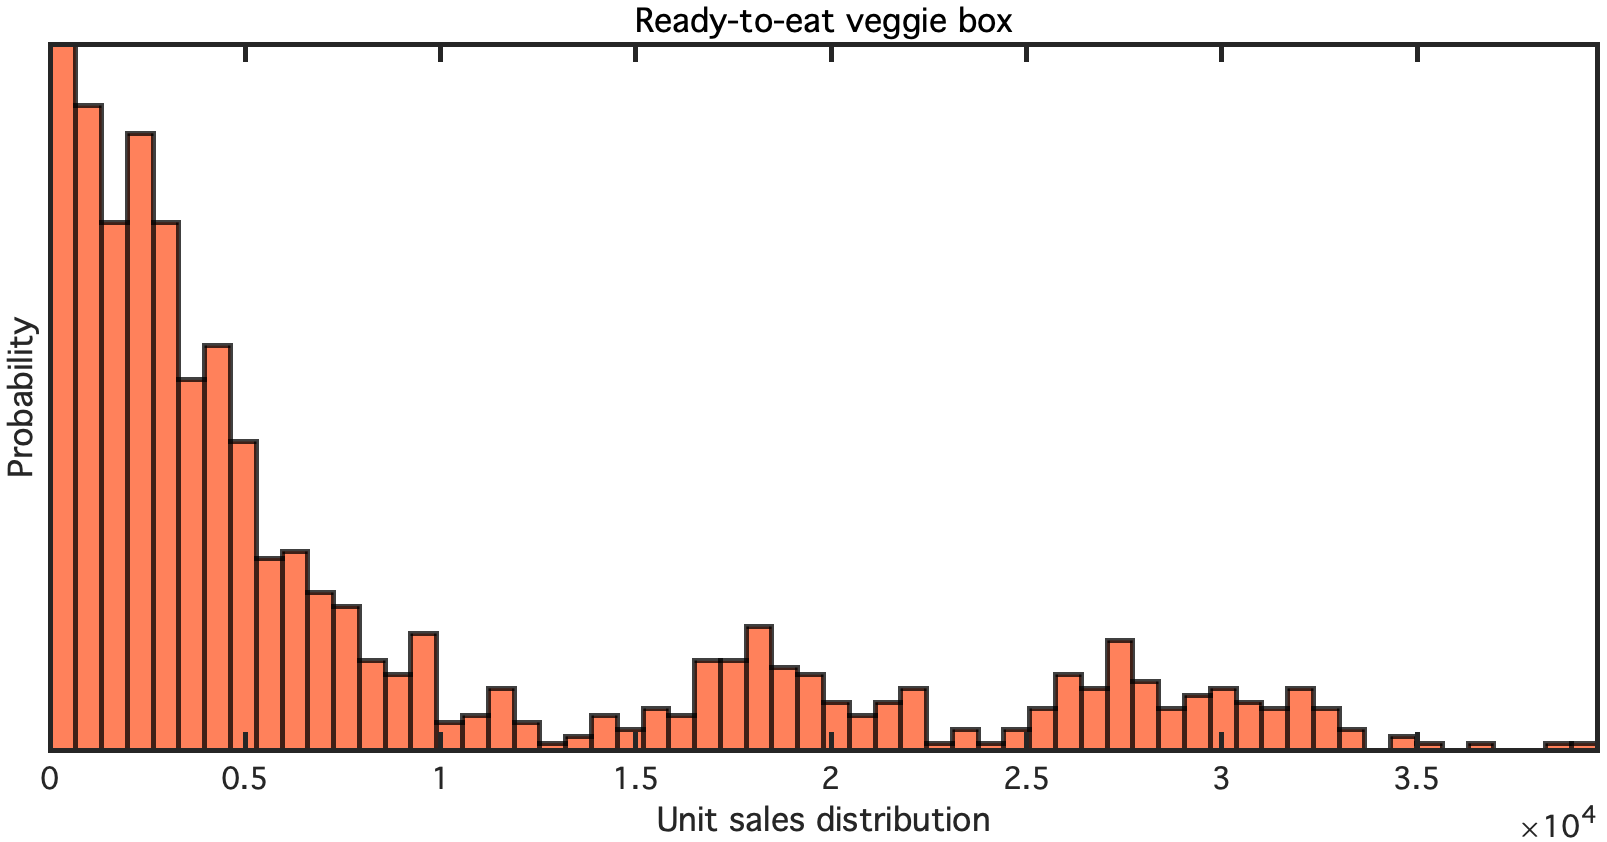
\includegraphics[width=\columnwidth]{figs/aguil4.png} 
      \caption{Distribution of sales during promotions of a model simulating a popular ready-to-eat vegetables box. The variability of promotional sales can be overwhelming.}
\label{fig:fakeProduct}
\end{figure}


We have invested extensive time in understanding this promotional product as well as recreating its sales through a known mixture model. The variables of the model are the following: variable $\mathbf{x_1}$ is drawn from the standard uniform distribution $\textit{U}(0,1)$ and it simulates the normalised discounts; variable $\mathbf{x_2}$ follows the exponential distribution $f(x;\lambda=1)=e^{-x},~x\geq 0$ and it accounts for the baseline sales; variable $\mathbf{z}$ simulates fat-tailed effects like store affluence, typically not captured by the retailers, and it is drawn from a Rayleigh distribution $f(x;\sigma)=\frac{x}{\sigma^{2}}e^{-x^{2}/(2\sigma ^{2})},~x\geq 0$, where we set the scale parameter $\sigma ={\sqrt {\frac {2}{\pi }}}$ to have unit mean. This variable $\mathbf{z}$ is the confounding one and it is partly present in the predictor variable $\mathbf{x_3}$, as it is defined as $\mathbf{x_3} = \mathbf{u_1} + \gamma \mathbf{z}$, where $\gamma = 0.15$, $\rho_{\mathbf{x_3}, \mathbf{z}} \neq 0$ and $\mathbf{u_1} \sim \textit{U}(0,1)$; variable $\mathbf{x_3}$ can be seen as an indicator of the number of times the shelf containing the product is replenished, which is a measurable quantity and partly influenced by the store affluence; variable $\mathbf{x_4}$ models the common linear dependence observed in retailing data. For example, the number of orders of the ready-to-eat vegetables box placed by the stores is related to the sales of the product itself. Therefore, let us define $\mathbf{x_4} = \lambda_0 + \lambda_1 \mathbf{x_2}$, so $\mathbf{x_4}$ and $\mathbf{x_2}$ are linearly dependant. Two categorical variables are also generated. The first one, $\mathbf{c_1}$, follows a Bernoulli distribution \textit{B}(1, p=0.5) and it can be seen as a variable indicating when the promotional product has been featured in a special display in half of the stores; variable $\mathbf{c_2}$ indicates that during the promotion, the stores were nearly out of stock and requested more units to the distribution centre. That variable is correlated with $\mathbf{x_2}$ and defined as $\mathbf{c_2} = (\mathbf{x_2} > 0.85)$.


After defining the input variables, let us introduce the mixing model that generates the 500 observations of sales $\mathbf{y}$. As per the real-market data that we have analysed, large discounts properly advertised tend to generate an avalanche effect in sales. To simulate this effect, variable $\mathbf{x_1}$ is mapped with an operator $\varphi(x)$ as defined next,
\begin{equation}
\varphi(x) = 
  \begin{cases} 
   1000+x & 0.5\leq x < 0.8 \\
   2500+x & 0.8\leq x < 0.9 \\
   3800+x & x \geq 0.9 \\
  \end{cases}
\label{eqn:mapping}
\end{equation}

The rest of the variables contribute to the response variable in different capacities as per,
\begin{equation}
y = \omega_1 \varphi(x_1) + \omega_2 x_2+ \omega_5 c_1+ \omega_6 c2 + \omega_7 z\\ 
\label{eqn:responseVar}
\end{equation}

We set the weights to $\mathbf{\omega} = [1,3100,0,0,10,0, 200]$. The largest weight, $\omega_2 = 3100$, has been calculated by fitting a exponential distribution to the actual sales of the ready-to-eat vegetables box. Note that variables $\mathbf{x_3}$, $\mathbf{x_4}$ and $\mathbf{c_2}$ do not contribute to the sales, but are part of the information collected by some retailers. To account for some imprecision in the model, such as events that occur at tilt level like double scanning, no-scanning, damaged products or refunds, we add some white noise to the sales signal, in our case $\mathcal{N}(\mu=46.5,\,\sigma^{2}=1.6 \cdot 10^6)$. The full model is summarised in Figure~\ref{fig:endogeneitySummary}.

\begin{figure}
    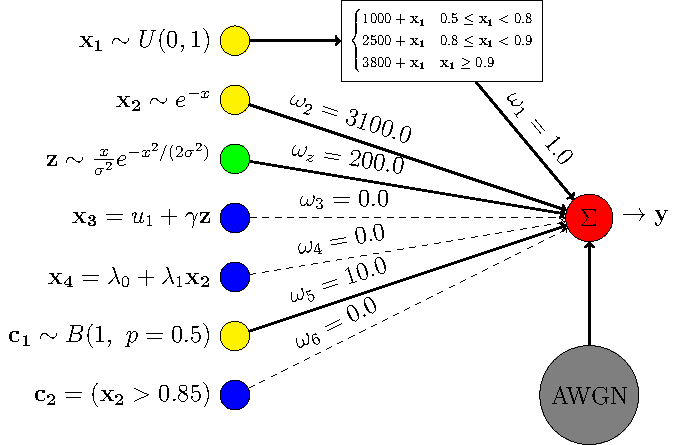
\includegraphics[width=\columnwidth]{figs/aguil5.pdf}
\caption{Illustration of the data model: yellow nodes represent independent variables, blue ones are collineal variables and the green one is the confounding variable. The output variable $\mathbf{y}$ represents the sales in units. Variable $\mathbf{x_1}$ is mapped to represent the sales avalanche effect that large discounts produce. Variables $\mathbf{x_3}$, $\mathbf{x_4}$ and $\mathbf{c_2}$ do not contribute to the sales, hence their weights $\omega$ are zero.}
\label{fig:endogeneitySummary}

\end{figure}


As mentioned before, the first block of the experiment evaluates the method in an ideal scenario where only the variables that contribute to the response variable are observed, namely $\mathbf{x_1}$, $\mathbf{x_2}$, $\mathbf{c_1}$ and $\mathbf{z}$. 

The second block introduces collinearity in the information available for forecasting, therefore, besides the variables from block 1, variables $\mathbf{x_3}$, $\mathbf{x_4}$ and $\mathbf{c_2}$ are also part of the input dataset. Note that these collinear variables do not contribute to the response variable. The idea is to evaluate our method with rank deficiency conditions.

The third block aims to recreate endogeneity through the confounding variable $\mathbf{z}$, which in this setup affects $\mathbf{x_3}$ and $\mathbf{y}$, but it is not observed.

Table~\ref{tab:endogeinity} summarises the results of the experiments where our method produces decent results in all the scenarios, and the forecasting error measures used are described in \ref{app:ForecastErrors}. It is particularly noticeable that the performance of our method is affected by collinearity. The explanation is that the values of $\mathbf{v}$ are distributed across the variables as the method identifies $\mathbf{c_2}$, $\mathbf{x_3}$, and especially $\mathbf{x_4}$, as related to the response variable. That occurs because these variables are noisy representations of $\mathbf{x_1}$, $\mathbf{x_2}$ and $\mathbf{z}$, hence our algorithm is mislead when searching for similar promotions. On the other hand, endogeneity does not affect the performance too much, mainly because much information of the response variable is already captured in $\mathbf{x_1}$ and $\mathbf{x_2}$. A few fat-tailed promotions are not correctly predicted as these extreme values come from the confounding variable, but the increase in promotions outside 50\% is just 1.14\%.

\begin{table*}[t]
\centering
\resizebox{\textwidth}{!}{
\begin{tabular}{@{}cccccccccc@{}}
\toprule
\textbf{Case} & \textbf{Observed} & \textbf{method} & \textbf{$R^2$} & \textbf{frcError} & \textbf{frcBias} & \textbf{RMSE} & \textbf{MAPE} & \textbf{w20p} & \textbf{out50p} \\ \midrule

\multirow{2}{*}{ideal} & \multirow{2}{*}{$\mathbf{x_1}$,$\mathbf{x_2}$,$\mathbf{c_1}$,$\mathbf{z}$} & our method & 0.90 & 0.24 & 0.11 & 2886.69 & 178.52 & 54.06 & 7.07 \\
 &  & LS & 0.58 & 0.64 & 0.02 & 6072.26 & 398.19 & 14.08 & 27.58 \\
\hline 
\multirow{2}{*}{collinearity} & \multirow{2}{*}{$\mathbf{x_1}$,$\mathbf{x_2}$,$\mathbf{x_3}$,$\mathbf{x_4}$,$\mathbf{z}$,$\mathbf{c_1}$,$\mathbf{c_2}$} & our method & 0.82 & 0.29 & 0.09 & 3915.33 & 159.98 & 50.32 & 8.65 \\
 &  & LS  & 0.58 & 0.64 & 0.02 & 6078.30 & 388.58 & 11.39 & 27.38 \\
 \hline
\multirow{2}{*}{endogeneity} & \multirow{2}{*}{$\mathbf{x_1}$,$\mathbf{x_2}$,$\mathbf{x_3}$,$\mathbf{c_1}$} & our method & 0.88 & 0.26 & 0.05 & 3233.96 & 225.02 & 55.61 & 8.21 \\
 &  & LS  & 0.58 & 0.64 & 0.03 & 6055.49 & 390.56 & 11.39 & 27.58 \\ 
\bottomrule
\end{tabular}
}
\caption{Collinearity and endogeneity experiment results. The ideal case refers to a forecast where no collinearity neither endogeneity conditions are present, as per the set of observed variables. In the second case, collinear variables are introduced and subsequently the performance of the method decreases. The third case depicts the situation where one of the variables that contributes to the sales is not observed, although a noisy version ($\mathbf{x_3)}$ is yet recorded. Description of each measure can be found in \ref{app:ForecastErrors}.}
\label{tab:endogeinity}
\end{table*}



%- - - - - - - - - - - - - - - - - - %
\subsection{Mother's Day Experiment} \label{subSect:MomsDay}

A common challenge for retailers is the forecast of events, defined as short periods of time where the volume of sales for some particular products massively increases. Mother's Day is a good example of it as during this event customers almost compulsively buy gifts such as flowers or chocolates, increasing the average sales in orders of magnitude. The idea behind this first experiment is to mock the sales of an imaginary product as the combination of some of the input variables and to represent Mother's Day as an increase in sales. This experiment is an example of the promotional subrepresentation illustrated in Eq.\eqref{eqn:nonuniform_sampling}.

Within this framework, the capabilities of the proposed method to infer the mechanisms behind promotional sales are evaluated. The goals of this experiment are therefore, to evaluate if the method is       able to identify the variables contributing to the sales. Also, to assess the impact of the free parameters number of iterations and size of training bag in this controlled experiment, and finally, to get a comparison between bagging and the fast subsampling approach proposed at the end of Section \ref{sect:Model}.

The toy dataset which models Mother's Day consists of a matrix $\mathbf{X} = ( \mathbf{X_{num}} \cup \mathbf{X_{cat}} ) \in \mathbb{R}^{N \times (I+J)}$ where the $I$ numerical variables $\mathbf{X_{num}} \in \mathbb{R}^{N \times I}$ are drawn from a uniform distribution \textit{U}(0,1) whereas the categorical data $\mathbf{X_{cat}} \in \mathbb{R}^{N \times J}$ come from a Bernoulli distribution \textit{B}(1, p=0.5). 

The promotional sales $\mathbf{y} \in \mathbb{R}^{N \times 1}$ are generated as the combination of $I$ numerical variables, $J$ categorical variables and white noise. The contribution of each variable is defined by a mixing column vector $\boldsymbol{\gamma}=[\alpha_1,\ldots,\alpha_I,\beta_1,\ldots,\beta_J]^\top \in \mathbb{R}^{(I+J) \times 1}$ where $\alpha_i \in (0, 100)$ and  $\beta_j \in \{0, 1, 2, \ldots, 100\}$. The noisy addition is a column vector $\mathbf{g} \in \mathbb{R}^{N \times 1}$ where each observation $g_n$ is normally distributed with $\mu = 0$ and $\sigma^{2} = 10$. The response variable is thereby  generated as $\mathbf{y} = \mathbf{X}\boldsymbol{\gamma} + \mathbf{g}$.

% From here, define how the data was used for the experiment
Using this setup, let us generate 500 random samples of the toy dataset with 5 numerical ($n_i$) and 5 categorical variables ($c_j$), where the sales are the combination of only 3 of those variables. To introduce 4 Mother's Day events in the dataset, we randomly select 4 samples and boost the sales by adding 3 times the averaged sales in the dataset (117.17). To flag these days, a binary variable $md$ is introduced and always set to false apart from these 4 days where the sales get 117.17 units increased. The equation that generates the mock sales is $y = 0.08 ~ n_1 + 0.16 ~ c_1 + 0.15 ~ c_3 + 0.61 ~ md$, where the coefficients have been normalised. % and the data is depicted in Figure\ref{fig:fsMockSales}.  
The evaluation of the accuracy of the feature selection is calculated as the sum of absolute error $\delta$ between the actual feature importance and the calculated feature importance vectors, both normalised to 1.0. To benchmark the quality of the feature selection with another model, we compare it to an ensemble of Least-squares boosting (LSBoost) regression trees. \myblue{The ensemble consists of 100 LSBoost trees with a learning rate of 1.0, trained on the same Mother's Day data than our method.}


During the tests, the size of the training bag was swept from 25\% to 50\%, whereas the number of iterations ranged from 500 to 1000. All the combinations were able to correctly identify the variables that drive the sales, although the importance assigned to the Mother's Day variable is larger than it should when using sampling bags of 50\%. Duplicating the number of iterations in bagging does not produce any improvement but it does increase the computational burden. In this sense, the gap between subsampling and bagging is quite large, although both approaches give very similar results. Figure \ref{fig:baggingSubsampling} shows a comparison between the two aforementioned strategies, where the top row represents the features selected in each iteration and the bottom row corresponds to the averaged results. The values have been normalised from zero to one and the color scale maps zero values to light blue. Inspecting the figure shows that both approaches select $md$ as the most relevant feature followed by $c_1$, $c_3$ and $n_1$, disregarding the remaining variables.
%
\begin{figure*}[t]
      \centering
       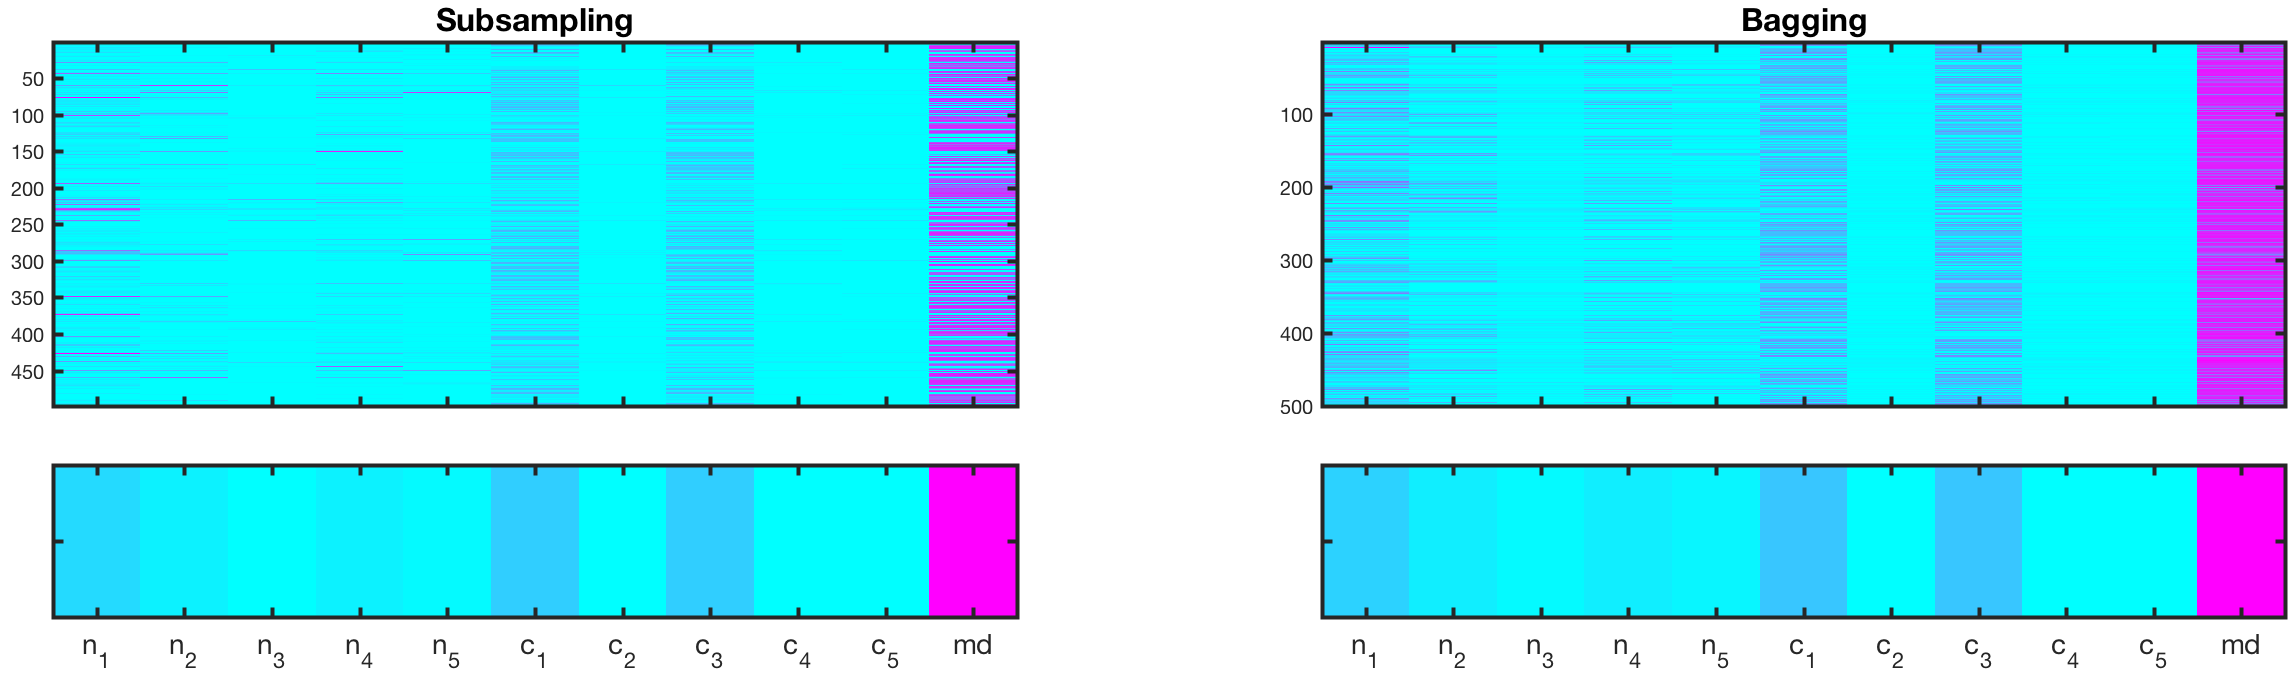
\includegraphics[width=\textwidth]{figs/aguil6.png} 
      \caption{This figure depicts the two Feature Selection approaches described in this paper: left column is sub-sampling (Algorithm \ref{alg:2}) and right column shows traditional bagging (Algorithm \ref{alg:1}) applied to the Mother's Day dataset. The top row shows the iterations (y-axis) vs the value of the features (normalised from 0 to 1) and the bottom row shows the average of the iterations. Light blue means zero whereas light pink represents the higher score in the feature selection. The results obtained with the sub-sampling method are very similar to bagging at a lesser computational burden. Both approaches select $md$ as the most relevant feature followed by $c_1$, $c_3$ and $n_1$, disregarding the remaining variables.}
\label{fig:baggingSubsampling}
\end{figure*}
%
%
For this application, bag-sizes of 25\% produce better results than 50\%, and subsampling is substantially quicker than bagging. The variable importance vector calculated by the 100 decision trees is a bit far from the actual ones, being the absolute error $\delta=0.30$, as the variable $md$ gets nil importance.
%
\begin{figure*}[t]
  \centering 
  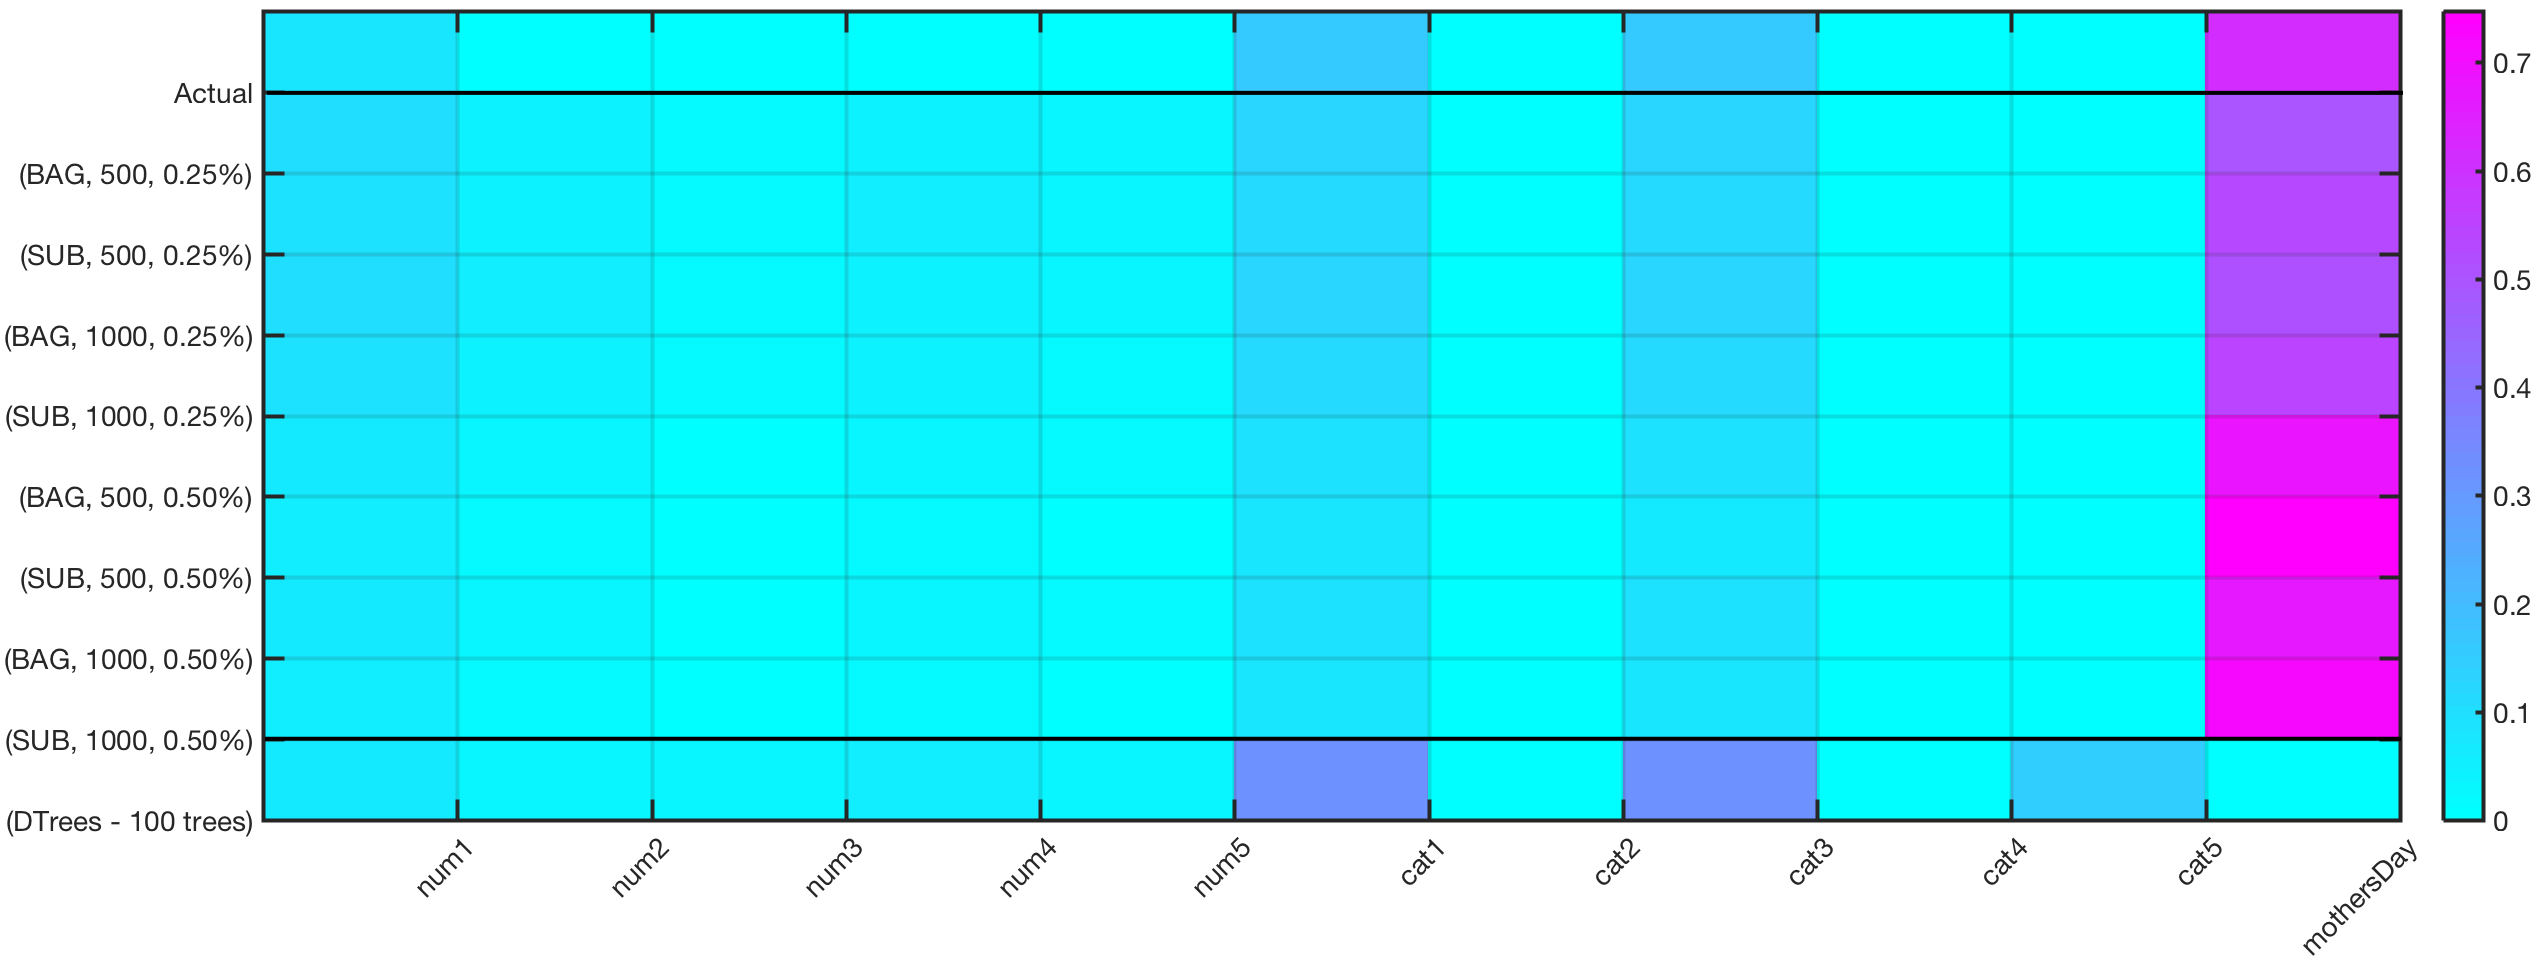
\includegraphics[width=\textwidth]{figs/aguil7.png} 
  \caption{Feature Selection for events: Mother's Day example. The grid shows the variable importance where the closer to blue light is the least important. Top row represents the actual variable importance of the surrogate model. Following rows correspond to the different settings of our method and bottom row represents the outcome of a 100 decision trees model. In this experiment, only 4 of the 11 variables contribute to the sales as per the following equation $y = 0.08 ~ n_1 + 0.16 ~ c_1 + 0.15 ~ c_3 + 0.61 ~ MD$. All of the methods successfully identify $c_1$ and $c_3$, although the combinations with a bag of 50\% assign too much importance to $md$ variable (totally neglected by the DT model). The best approach is subsampling with a bag of 25\% over 1000 iterations.}
  \label{fig:fsVarImportance}
\end{figure*}
%
A decent interpretation of this experiment is provided in Figure \ref{fig:fsVarImportance}, where the features are represented in a grid coloured by variable importance. The first row holds the actual values of the toy dataset and the last one is the results using decision trees. The similarity between the first row and the remaining ones indicates how accurate the feature importance selection is, where the cells in light blue are valued zero. 
%
\begin{table*}[t]
 \centering
\resizebox{0.8\textwidth}{!}
{\begin{tabular}{ccccccccc}
\toprule
Iterations & bagSize & absError  & $\tau(s)$ & Method & $n_1$ & $c_1$ & $c_3$ & MD \\
\midrule
  &  & & & \textbf{ACTUAL} & \textbf{0.08} & \textbf{0.16} & \textbf{0.15} & \textbf{0.61} \\
 \hline
 500 & 0.25 & 0.37 & 39.19 & BAG & 0.10 & 0.12 & 0.12 & 0.50 \\
 500 & 0.25 & 0.35 & 0.99 & SUB & 0.09 & 0.11 & 0.11 & 0.53 \\
 1000 & 0.25 & 0.37 & 49.84 & BAG & 0.10 & 0.12 & 0.12 & 0.50 \\
 \textbf{1000} & \textbf{0.25} & \textbf{0.30}  & \textbf{1.39} & \textbf{SUB} & \textbf{0.09} & \textbf{0.11} & \textbf{0.11} & \textbf{0.55} \\
 500 & 0.50 & 0.31  & 28.32 & BAG & 0.06 & 0.09 & 0.09 & 0.68 \\
 500 & 0.50 & 0.41  & 0.59 & SUB & 0.05 & 0.07 & 0.07 & 0.75 \\
 1000 & 0.50 & 0.31  & 56.46 & BAG & 0.06 & 0.09 & 0.09 & 0.68 \\
 1000 & 0.50 & 0.37 & 1.42 & SUB & 0.05 & 0.08 & 0.08 & 0.72 \\
 \hline
  &  & 1.24  & 0.85 & DT (100) & 0.06 & 0.32 & 0.32 & 0.00 \\
\bottomrule
\end{tabular}}
\caption{Feature Selection for event-driven mock sales. First row represents the actual surrogate model $y = 0.08 ~ n_1 + 0.16 ~ c_1 + 0.15 ~ c_3 + 0.61 ~ MD$. The remaining rows show the combination of iterations, size of bag and type of sampling along with the results. The fifth row shows the best results in terms of absolute error. The bottom row shows the results of a 100 decision tree model.} 
\label{tab:Feature Selection}
\end{table*}

The positive result of this experiment shows that the method is robust and accurate in finding the main features driving sales, even if one of the most important effects increasing sales is only observed 4 times in the dataset of 500 samples. It also proves that the approach described in Algorithm \ref{alg:2} is powerful, reliable and faster than traditional bagging for this type of problems. 





%- - - - - - - - - - - - - - - - - - %
\subsection{Hyperparameter Tuning} \label{subSect:HyperParams}

% composition of several layers
% parameters whose values


As in the majority of machine learning methods, the one presented in Section \ref{sect:Model} produces different models upon the combination of the free parameters. The values to be set prior to the execution of the algorithm are summarised as follows:

\begin{itemize}
\item The bag size is the percentage of the training set used in the bagging or subsampling process.
\item The number of loops are a proxy to calculate the number of iterations as the size of the training set depends on the item to forecast for. Whereas some products are popular promotional items with many historical records, some of them might have rarely been on promotion. To deal with this spread, the number of training iterations are calculated as the product between the number of records in the training bag and the number of loops.
\item As discussed in Section \ref{sect:Model}, the features can be selected using bagging or sub-sampling, but also they can be selected through the combination of weak learners (WL) into an ensemble, typically with different hyperparameters to exploit diversity. We have also mentioned that instead of combining the selection of features, it is also possible to combine the predictions of each individual forecaster, and following the naming convention we refer to this approach as weak forecasters (WF). Let us refer to these options during the experiment as type of aggregation.
\item Finally, the number of neighbours can be determined either by cross-validation or by using a simple cut-off to 90\% of the cumulative sum of the weights.
\end{itemize}

%a ensemble of weak learners \ref{subsect:WL}
%   \ref{subsect:WF}.
To optimise the set of hyperparameters, real data from a retailer in a European country is used in a grid search. This dataset contains a medley of 354 products representing all food categories, beauty and household products, and drinks. The test set contains 361 nation-wide promotions to forecast for. On average, there are $18.72 \pm 8.92$ historical promotions per product running on $718.58 \pm 619.82$ large-medium-size stores (min 1, max 1738). There are no promotions with zero or negative sales.

Evaluating a forecast algorithm is not trivial at all. A classical forecast accuracy measure is the Mean Absolute Percentage Error (MAPE), as defined in \ref{app:ForecastErrors}, which gives an idea of the error but does not consider the volume of sales. From the business point of view, supply chain managers typically concern about the volume of forecast, mainly because of the costs and complexities associated with delivering. To model this effect, we focus on the forecast volume that deviates less than 20\% from the actual sales, and also, about the one that deviates more than 50\%, as the impact of such forecast errors is critical to the business. Both calculations are derived from the relative error between predicted $\hat{y}$ and actual sales $y$, defined as $\delta = 100\%\times \left|{\frac {y-\hat{y}}{y}}\right|$, where $\delta_{w20p} \leq 20\% $ and $\delta_{out50p} > 50\%$ are respectively, the 20\% and 50\% error bands. The actual sales of the  products contained in these bands are then used to produce the percentage that measures the volume retained in them with respect to the total volume of sales. The reason to include business metrics can be easily explained through the following example. Let the actual sales of 4 different products be $sales = \left[1, 10, 100, 10000, 20000\right]$, and the prediction just one more unit than the sales, i.e., $predicted = 1 + sales$. The MAPE is 22.2\% whereas the volume contained within 20\% is 99.99\%. Broadly speaking, when it comes to loading the pallets into a lorry, it is advisable to keep the business metrics in mind.

In order to rank the results of this experiment, let us introduce a score that combines business and forecast error measures, and also the response time. In retail chains, the predictions are reviewed by forecasters, and in many occasions modified according to their criteria. As mentioned earlier in this paper, this algorithm is designed to be to some extent interactive with the forecasters. Once the method has learned the features and produced a prediction, a forecaster can select or unselect the historical promotions used to forecast, or even change their contribution to the forecast by modifying weights $\mathbf{w}$. To factor the interaction in, the response time of the algorithm, measured as the average time per prediction, is also taken into account.

To produce a score using these four parameters, let us reuse Eq.\eqref{eqn:featuresMatrix}. In this scenario, $\mathbf{X'} \in \mathbb{R}^{m \times 4}$ contains a row per test and $\mathbf{x}$ is the ideal case with values $[t,out50p,w20p, MAPE] =[0,0,100,0]^T$. The actual score is calculated as the Euclidean Distance standarised by the standard deviation,

\begin{equation}
\mathit{eucScore} = (\mathbf{X'}-\mathbf{x}^k~\mathbf{1}^\top)~\mathbf{V}^{-1}~(\mathbf{X'}-\mathbf{x}^k \mathbf{1}^\top)^\top
\label{eqn:eucScore}
\end{equation}
%
Let us develop a explanation of the experiment by depicting the outcome in space (MAPE has been omitted) as in Figure \ref{fig:HyperParameters}. 
\begin{figure}[t]
      \centering
      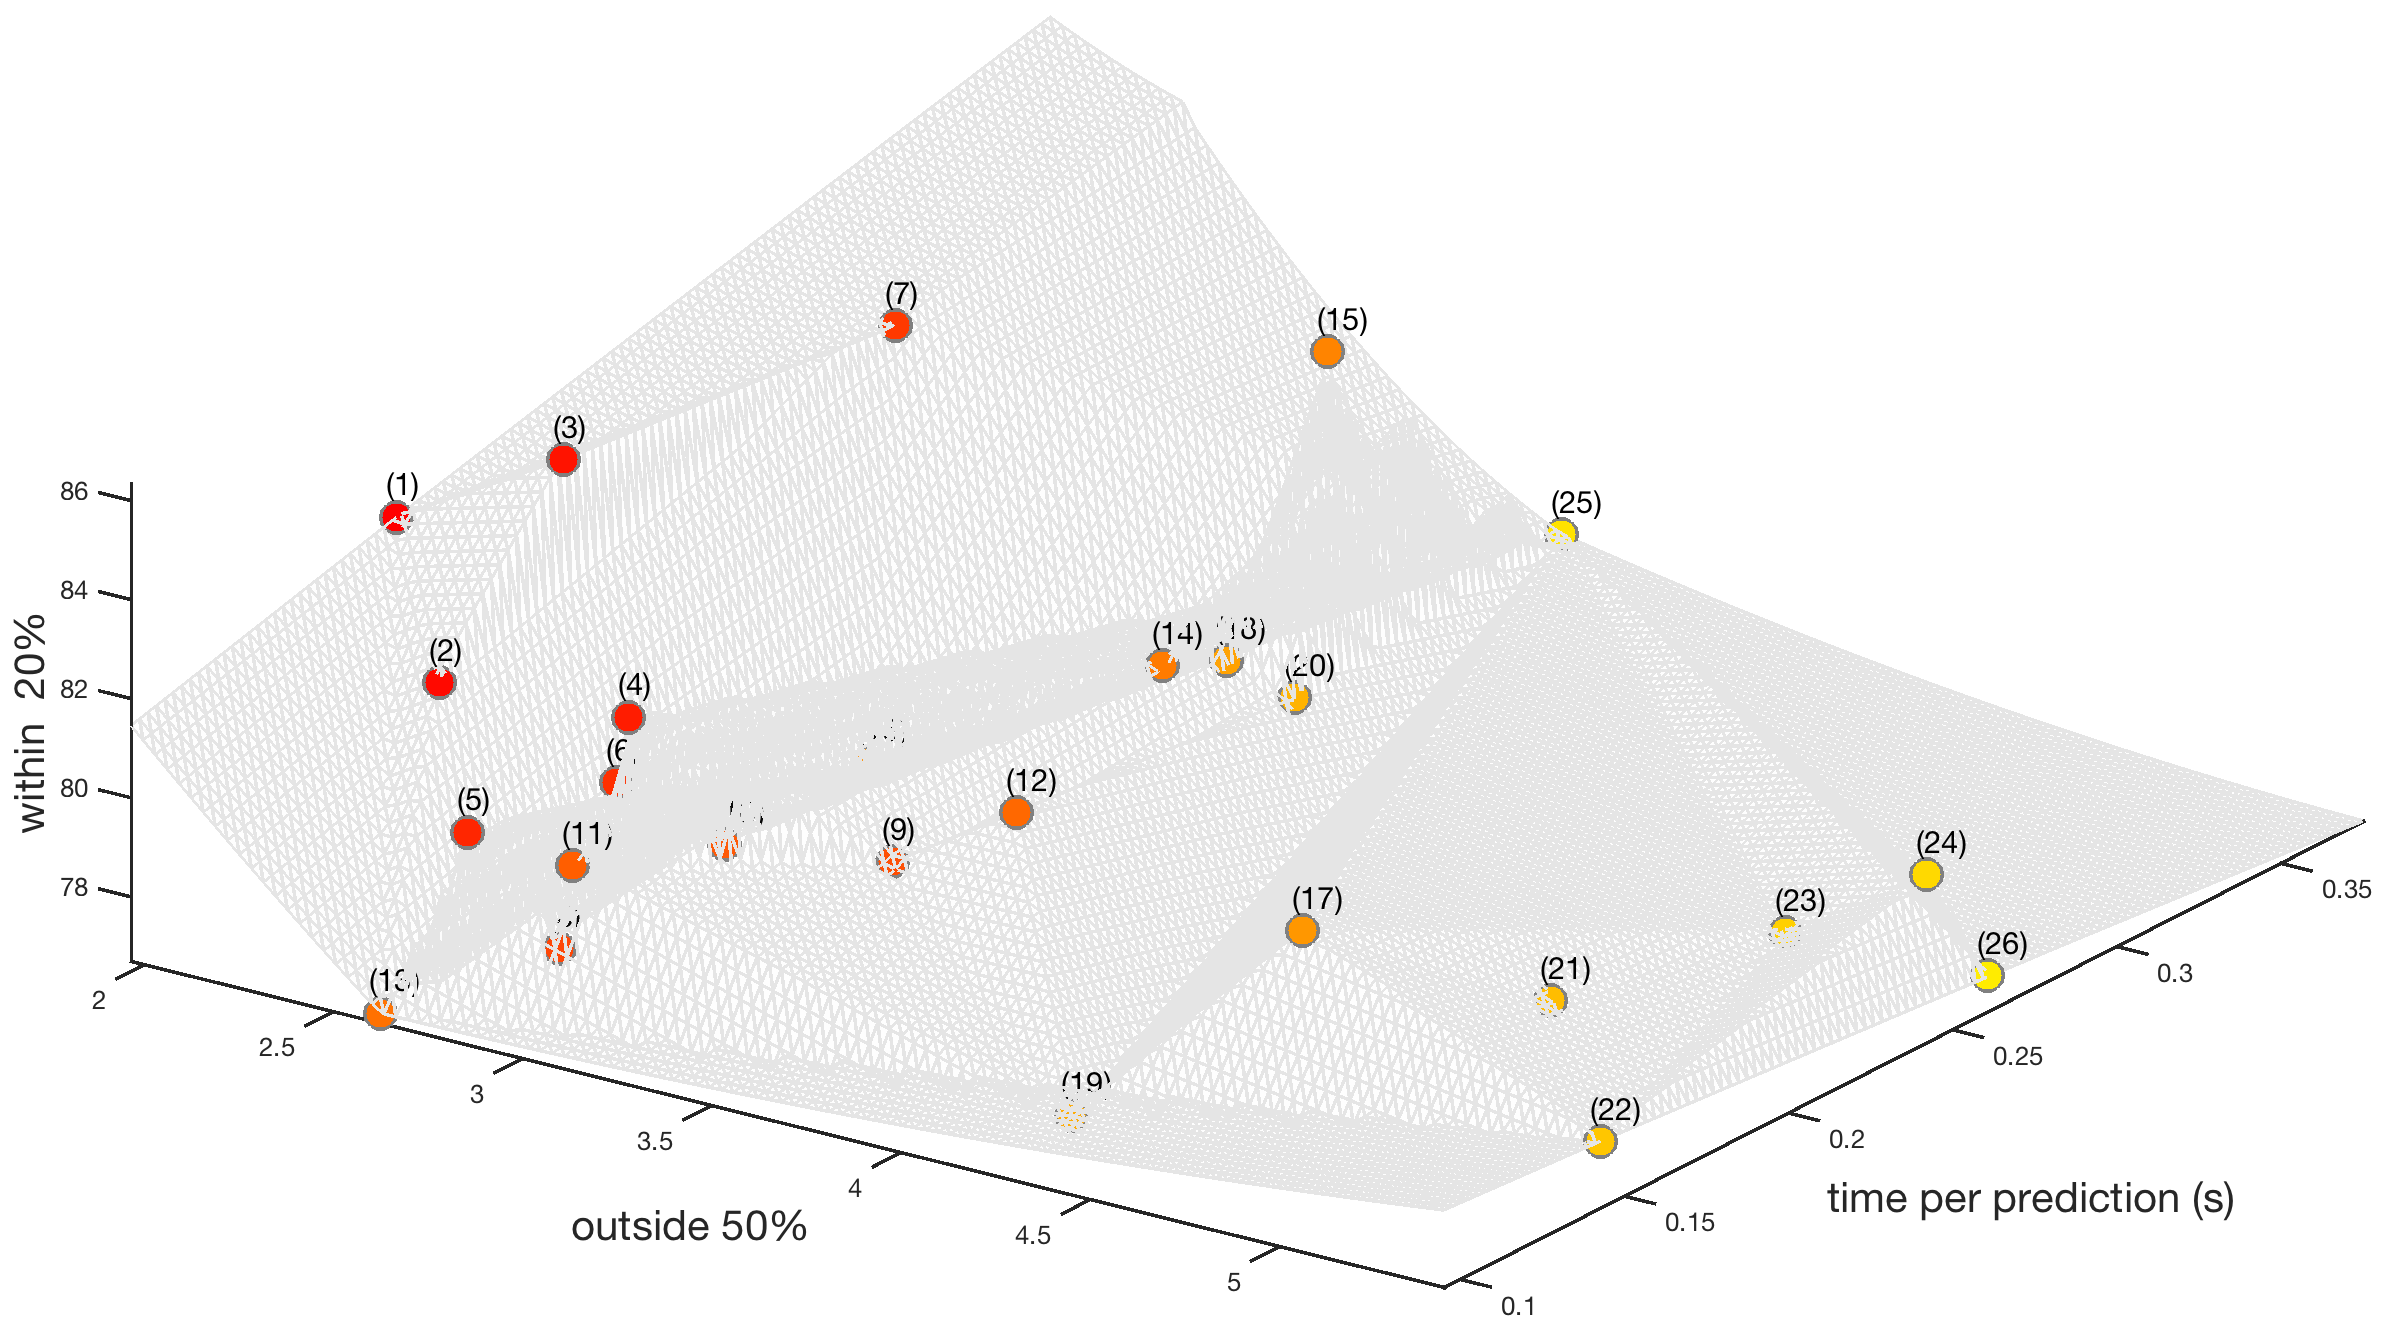
\includegraphics[width=0.5\textwidth]{figs/aguil8.png} 
      \caption{Tuning model hyperparameters: results of the parameter sweep considering the volumes within 20\%, outside 50\% and the computational time. The points are sorted by ranking score and each test is fully explained in Table \ref{tab:Hyperparameters}.}
      \label{fig:HyperParameters}
\end{figure}
%
Besides the points representing each test are well scattered over the space, the performance of the method does not dramatically change due to the different settings, proving that the method is robust. Also, the majority of the points lie in a region where the percentage of promotions outside 50\% of the error is low. Table \ref{tab:Hyperparameters} summarises the combinations of hyperparameters and the outcome in terms of the score and its four parameters, sorted from the smallest to the largest score. The top two ranking positions belong to ensemble of two WL, trained with a bag of 50\%, and 2 loops, where the one with cross-validated number of neighbours ranks first.
%
\begin{table*}[!htbp]
 \centering
\resizebox{\textwidth}{!}{\begin{tabular}{cccclrrrr}
\toprule
Ranking & eucScore & Bag Size & Num Loops & Aggregation & w20\% & out50\% & MAPE & $\tau$ (sec)\\
\midrule
 \textbf{1} & \textbf{1.26} & 5\textbf{0,50} & \textbf{2,2} & \textbf{WL ensemble + subsampling + CV} & \textbf{82.95} & \textbf{1.96} & \textbf{35.77} & \textbf{0.18} \\
 2 & 1.31 & 50,50 & 2,2 & WL ensemble + subsampling + NRG & 81.31 & 2.33 & 36.84 & 0.15 \\
 3 & 1.32 & 50 & 2 & Bagging + CV & 84.47 & 2.32 & 40.13 & 0.19 \\
 4 & 1.34 & 50 & 2 & Subsampling + CV & 82.17 & 2.94 & 38.17 & 0.13 \\
 5 & 1.35 & 50 & 2 & Subsampling + NRG & 80.32 & 2.74 & 37.33 & 0.11 \\
 6 & 1.39 & 100,50 & 1,2 & WL ensemble + subsampling + NRG & 79.60 & 2.70 & 36.52 & 0.16 \\
 7 & 1.39 & 50,50 & 2,2 & WF combine + bagging + CV & 83.94 & 2.35 & 35.59 & 0.28 \\
 8 & 1.44 & 100 & 1 & Bagging + NRG & 77.77 & 2.86 & 37.24 & 0.12 \\
 9 & 1.46 & 50 & 2 & Bagging + NRG & 79.24 & 3.41 & 36.93 & 0.16 \\
 10 & 1.46 & 100,100 & 1,1 & WL ensemble + bagging + NRG & 78.20 & 2.87 & 37.36 & 0.17 \\
 11 & 1.47 & 100,100 & 1,1 & WL ensemble + subsampling + NRG & 79.62 & 2.92 & 42.69 & 0.12 \\
 12 & 1.47 & 25,50 & 2,2 & WL ensemble + subsampling + CV & 80.14 & 3.61 & 37.44 & 0.18 \\
 13 & 1.52 & 100 & 1 & Subsampling + NRG & 76.90 & 2.62 & 42.96 & 0.10 \\
 14 & 1.52 & 50,50 & 2,2 & WF combine + subsampling + NRG & 80.16 & 3.36 & 36.93 & 0.25 \\
 15 & 1.52 & 50,50 & 2,2 & WL ensemble + bagging + CV & 84.99 & 3.39 & 40.30 & 0.30 \\
 16 & 1.52 & 50,50,50 & 2,2,2 & WL ensemble + subsampling + NRG & 77.45 & 2.70 & 36.70 & 0.23 \\
 17 & 1.52 & 25,50 & 2,2 & WL ensemble + subsampling + NRG & 80.32 & 4.56 & 36.61 & 0.15 \\
 18 & 1.54 & 50,50 & 2,2 & WL ensemble + bagging + NRG & 79.87 & 3.40 & 36.95 & 0.26 \\
 19 & 1.58 & 25 & 4 & Subsampling + NRG & 76.95 & 4.21 & 37.93 & 0.12 \\
 20 & 1.58 & 25,50 & 2,2 & WL ensemble + bagging + NRG & 79.09 & 3.52 & 37.04 & 0.27 \\
 21 & 1.63 & 25,50 & 4,2 & WL ensemble + subsampling + NRG & 78.78 & 4.98 & 37.30 & 0.18 \\
 22 & 1.69 & 25,25 & 2,2 & WL ensemble + subsampling + NRG & 78.05 & 5.43 & 38.48 & 0.14 \\
 23 & 1.71 & 25,50 & 2,2 & WF combine + subsampling + NRG & 78.29 & 5.07 & 37.07 & 0.24 \\
 24 & 1.73 & 25,25 & 2,2 & WL ensemble + bagging + NRG & 79.28 & 5.29 & 37.53 & 0.26 \\
 25 & 1.73 & 25,50 & 2,4 & WL ensemble + bagging + NRG & 78.48 & 3.32 & 37.32 & 0.38 \\
 26 & 1.79 & 25 & 4 & Bagging + NRG & 77.42 & 5.43 & 37.59 & 0.26 \\
\bottomrule
\end{tabular}}
\caption{Summary of the parameter sweep used to tune the hyperparameters ranked by results score. The top ranking position belongs to an ensemble of 2 WL, trained with a bag of 50\% and 2 loops, and the number of neighbours has been cross-validated. CV stands for cross-validation and NRG means that the number of neighbours has been selected by  retaining 90\% of the energy of the weights.} 
\label{tab:Hyperparameters}
\end{table*}
%
As per the result of this experiment, the value of the hyperparameters to use in the remaining experiments are: a ensemble of 2 weak learners, the feature selection done by subsampling with bag sizes of 50\%, and 2 training loops. Finally, the number of neighbours is calculated by cross-validation from now on.
%- - - - - - - - - - - - - - - - - - %

\subsection{Market Data} \label{subSect:TescoData}

In this experiment we apply the method presented in this paper on actual market data provided by a worldwide retailer, setting the values of the hyperparameters as discussed in Section \ref{subSect:HyperParams}. These datasets from 2016 contain data from 3 different countries and all types of promotional products grouped into the following categories: packed food (1-3), confectionery, drinks (1-2), fresh food (1-5), frozen food, non-food items (1-3) and precooked. The loose naming convention aims to comply with confidentiality terms. The total number of promotions in the test set is 43757, whereas the training set is larger than a million records. The sales are aggregated by clusters of similar stores. The retailer has also kindly provided with its forecast, which it is used as a benchmark. As the sales for the market data present different orders of magnitude, we also use the Normalised Root Mean Squared Logarithmic Error (NRMSLE).

%, calculated as follows:
%\begin{equation}
%\mathit{NRMSLE} = \sqrt{\frac{1}{N}\sum_{i=1}^{N} \ln \left( \frac{1+\hat{y}_{i}}{1+ y_{i}} \right)^2}
%\label{eqn:NRMSLE}
%\end{equation}

Additionally, to compare our method to a publicly available academic one, a LSBoost ensemble with 100 trees is generated per category, being trained on the same data as our method. Table \ref{tab:datasets} summarises a comprehensive explanation of the datasets.
%
\begin{table*}[t]
 \centering
\resizebox{\textwidth}{!}{\begin{tabular}{ccccccccc}
\toprule
Dataset & Continent & Categories & Products & Types of Stores & Test set & Training set & Average stores & Average sales \\
\midrule
 1 & Europe & 11 & 1984 & 2 (small-medium) & 2532 & 90879 & 614.46 & 7337.35 \\
 2 & Europe & 12 & 7676 & 6 (medium-large) & 24640 & 933631 & 152.45 & 6473.06 \\
 3 & Asia & 9 & 3774 & 6 (all types) & 10231 & 94880 & 313.99 & 13712.72 \\
\bottomrule
\end{tabular}
}
\caption{Summary of the real promotional datasets.}
\label{tab:datasets}
\end{table*}
%
%
The three methodologies are evaluated using the score presented in the previous experiment, although the computational time is not available for the retailer's forecast data, so it is excluded from the calculation.

% Express
The first dataset represents small-medium size stores in a European country with 1984 different products from 11 categories amongst the 14 overall available. The results show that our method outperforms both decision trees and the benchmark, especially in the categories fresh-1 and packed-food 2, where the method performs exceedingly well and 83\% of promotions lie within 20\% of the forecast error - the benchmark is above 75\% for these categories. For the rest of the categories, the method performs above the benchmark on a narrower margin. Figure \ref{fig:resultsAllCountries} shows the comparison between the three approaches sorted by the score of the benchmark. Although the performance of the 100 decision trees model is acceptable, the score is quite far out from the other techniques. Table \ref{tab:GlobalResults} shows a breakdown of different indicators for the 3 approaches at an aggregated level. Let us inspect MAPE and NRMSLE from rows 5 and 7 to illustrate why it is not advisable to use just one type of parameter to judge a forecast technique.  By looking at MAPE values, the forecast in the $7^{th}$ row gets a better score than row number 5, and even the NRMSLE values are arguably close, but the percentage of forecast with a larger error than 50\% adds up to almost 30\%, which translates into inadequate and costly supply chain processes.
%

\begin{figure}[t]
      \centering
\resizebox{\columnwidth}{!}{
 \begin{tabular}{c}
      %\includegraphics[width=\textwidth, height=0.25\textheight]{figs/resultsUKExpress.png} 
      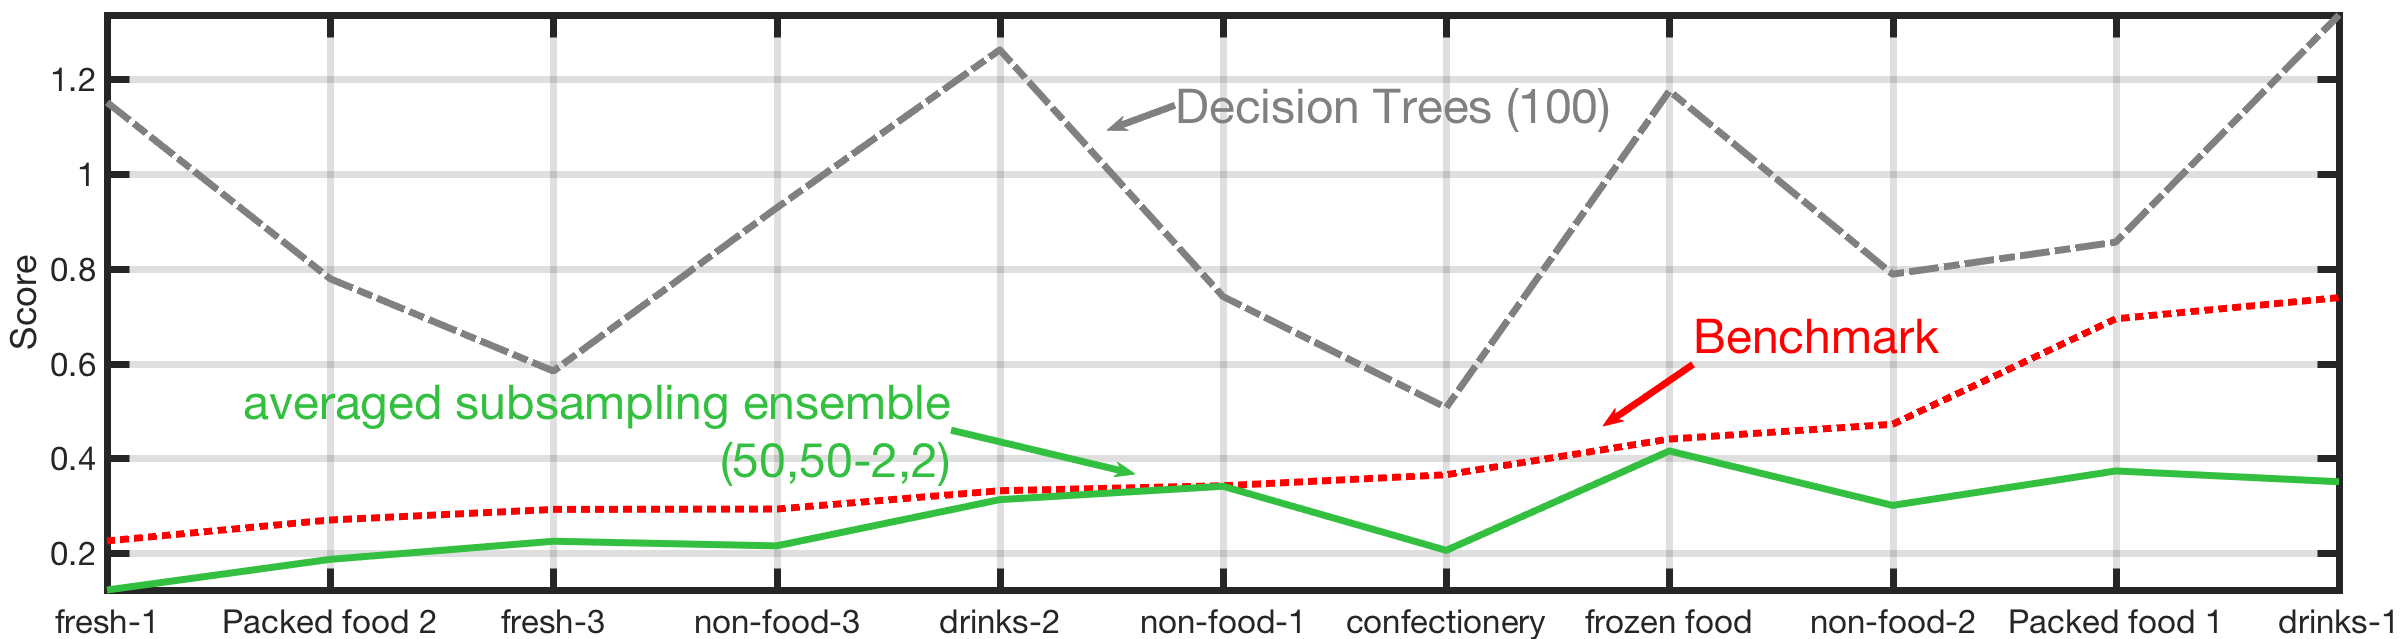
\includegraphics[width=.8\textwidth]{figs/aguil9.png} \\ %(a) Dataset 1. Small-medium size stores for a European country.\\
      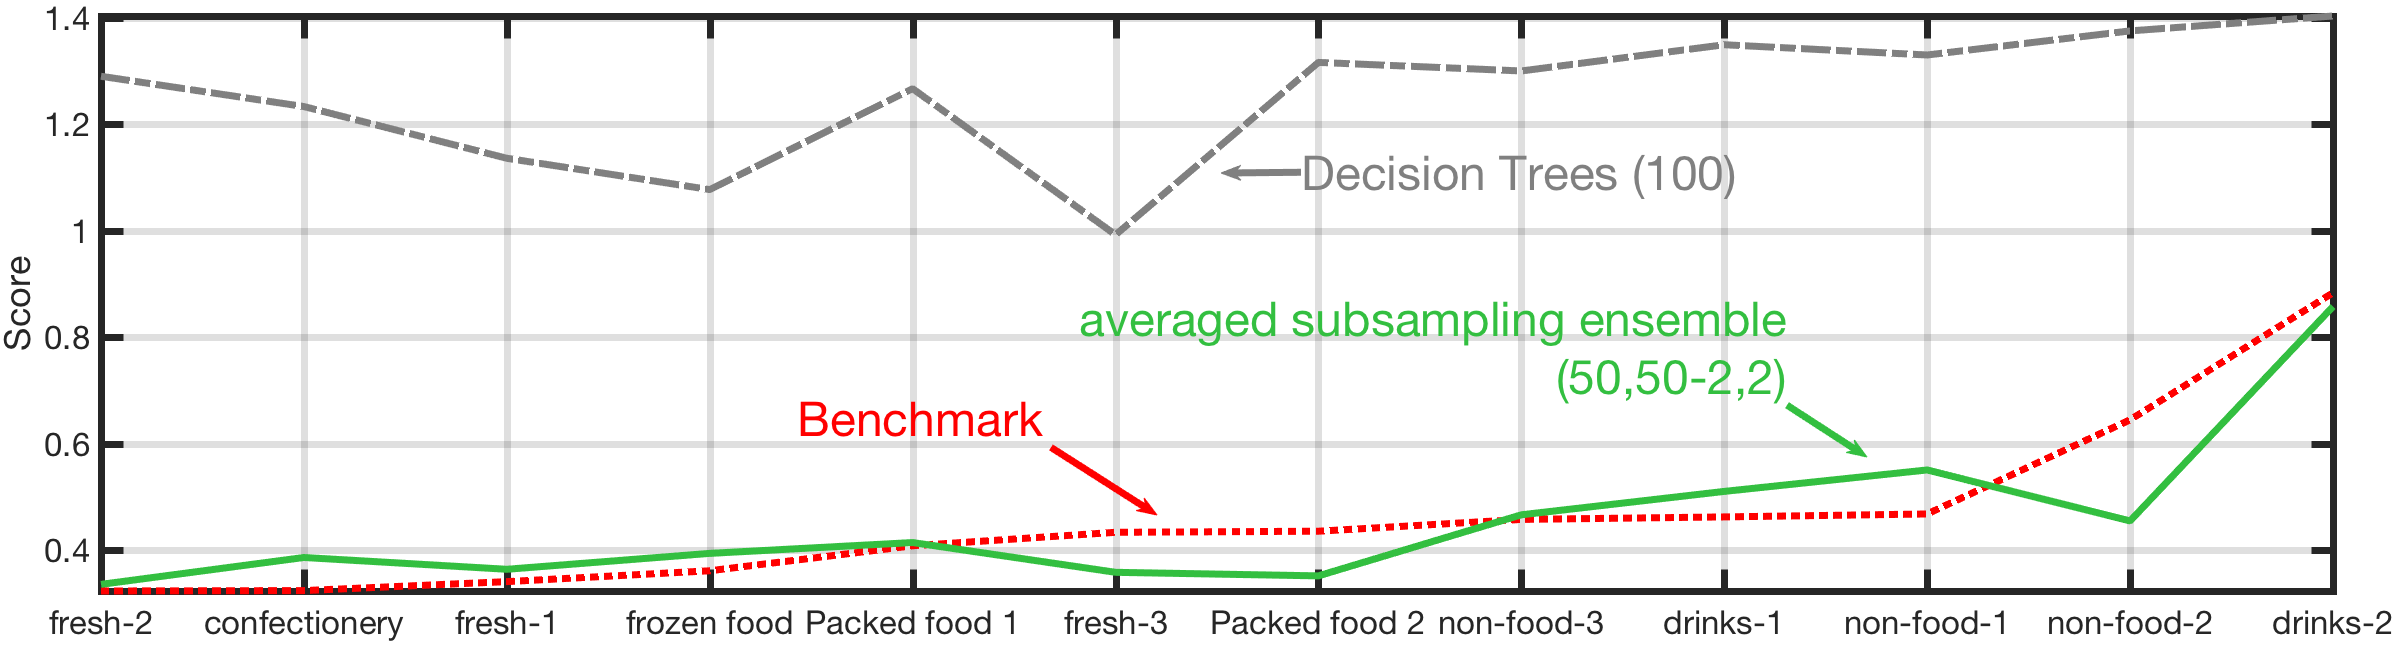
\includegraphics[width=.8\textwidth]{figs/aguil10.png} \\ %(b) Dataset 2. Medium-large size stores for a European country.\\
      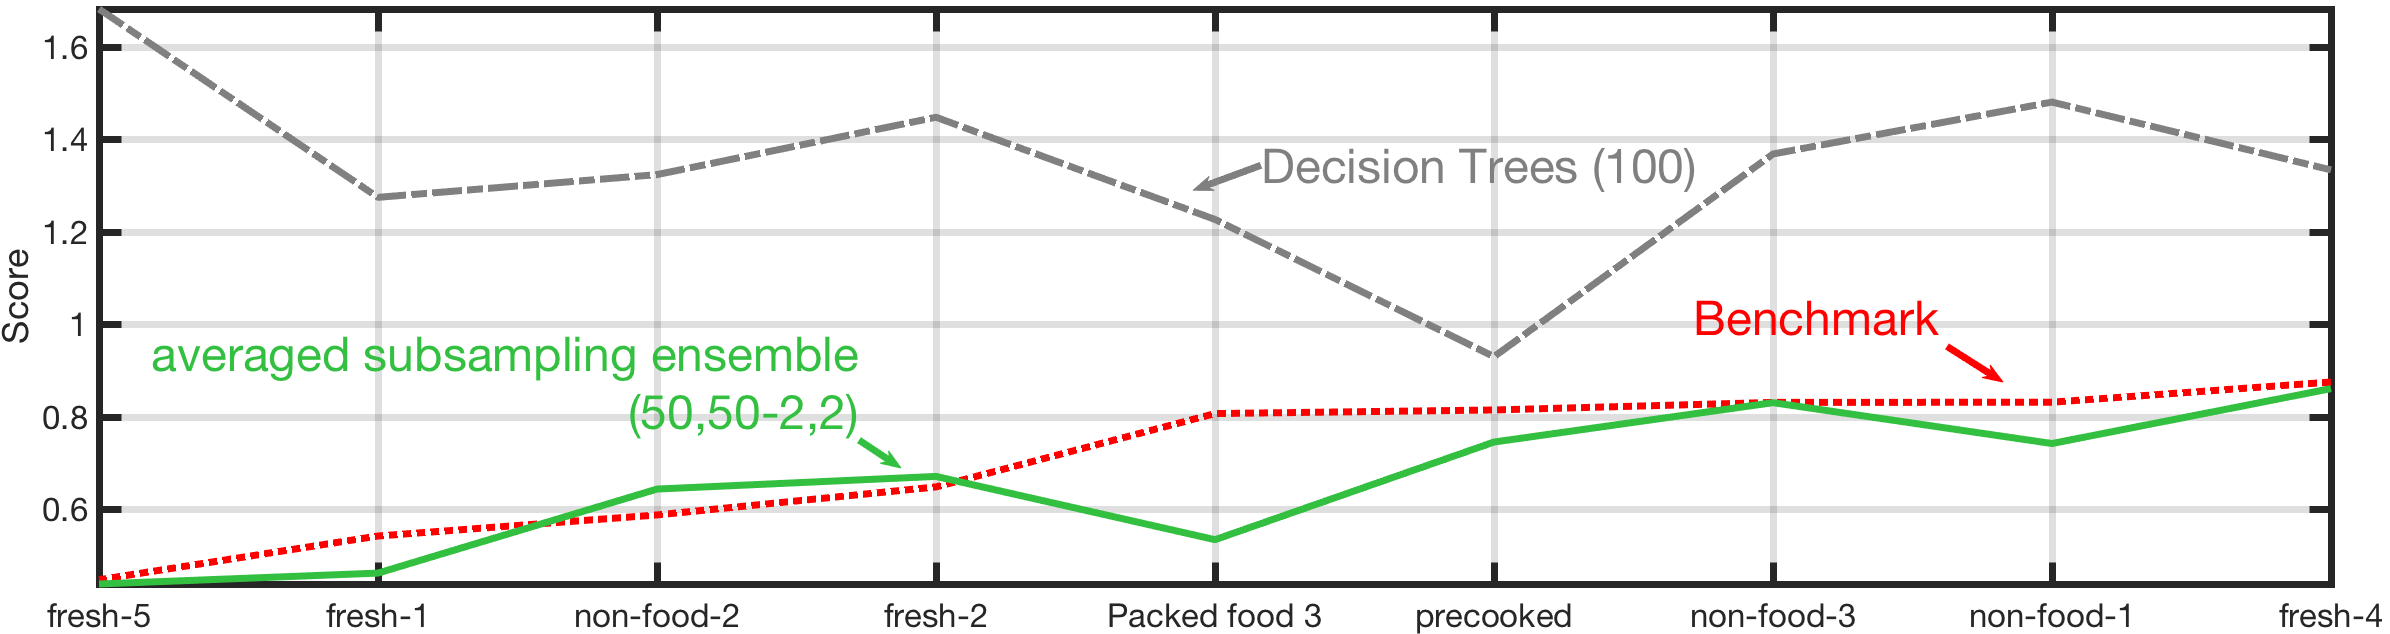
\includegraphics[width=.8\textwidth]{figs/aguil11.png} %\\ (c) Dataset 3. All store types stores for Asian country.\\ 
 \end{tabular}}
      \caption{Comparison between the accuracy score (lower is better) of method presented in this paper (green line), decision trees (gray dashed line) and the benchmark (red points) for 3 real-market datasets. The top chart corresponds to Dataset 1, small-medium size stores for a European country. The middle one is Dataset 2, medium-large size stores for a European country and the bottom one is Dataset 3, all store types stores for Asian country. The results are sorted by ascending benchmarks' score (lower is better).}
\label{fig:resultsAllCountries}
\end{figure}

%
\begin{table}[t]
\centering
\resizebox{0.5\textwidth}{!}{ 
\begin{tabular}{clccccc}
\toprule
Row & Approach & Dataset & w20 & out50 & MAPE & NRMSLE \\
\midrule
1 & Our method  & DS1 & 75.61 & 3.84 & 42.21 & 0.40 \\
2 & Benchmark & DS1 & 68.28 & 7.06 & 60.93 & 0.50 \\
3 & Regression Trees & DS1 & 42.85 & 18.09 & 334.39 & 0.84 \\
 \hline
4 & Our method  & DS2 & 60.62 & 10.60 & 41.01 & 0.44 \\
5 & Benchmark & DS2 & 62.06 & 10.16 & 60.17 & 0.55 \\
6 & Regression Trees & DS2 & 25.89 & 37.00 & 281.43 & 1.15 \\
 \hline
7 & Our method  & DS3 & 34.28 & 27.49 & 53.33 & 0.57 \\
8 & Benchmark & DS3 & 34.07 & 29.24 & 63.57 & 0.73 \\
9 & Regression Trees & DS3 & 18.83 & 53.24 & 1152.40 & 1.73 \\
\bottomrule
\end{tabular}}
\caption{Comparison between methods for the 3 real datasets. The results are aggregated by the number of promotions and show that our method outperforms both the benchmark and regression trees in the 3 scenarios.} 
\label{tab:GlobalResults}
\end{table}

% $\mathit{NRMSLE}$ is calculated as $\sqrt{\frac{1}{N}\sum_{i=1}^{N} \ln \left( \frac{1+\hat{y}_{i}}{1+ y_{i}} \right)^2}$

%$\sqrt{\frac{1}{N}\sum_{i=1}^{N} \ln \left( \frac{1+\hat{y}_{i}}{1+ y_{i}} \right)^2}}%$
%\mathit{NRMSLE} = \sqrt{\frac{1}{N}\sum_{i=1}^{N} \ln \left( \frac{1+\hat{y}_{i}}{1+ y_{i}} \right)^2}
%\begin{equation}%\label{eqn:NRMSLE}} 

% UK
The second set consists of medium-large stores in a European country and it contains 7676 promotional products and 6 types of stores. It is worth mentioning that this dataset contains a wide spectrum of all of the promotional items: different selling rate products, so called fast, medium and slow sellers, bundled items, rebates, club-cards, products with very little or even no promotional history, amongst many others. In this aspect, the authors would like to stress that to tackle this variety of problems, grocers typically employ different algorithms whereas we are using the same method for all of these scenarios. That is the reason that in this experiment, our algorithm does not outperform the benchmark in all of the categories. As shown in Figure \ref{fig:resultsAllCountries}, the method performs above the benchmark for categories fresh-3, packed food-2 and non-food 2 and performs alike for packed food-1 and non food-3. These categories represent 62\% of this dataset, so when the results are aggregated per number of promotions, the figures favour our method. In the categories where our method underperforms the benchmark, the scores are decently close.% Decision Trees are in the limbo of forecast.


\begin{figure}[t]
      \centering
 \begin{tabular}{c}
      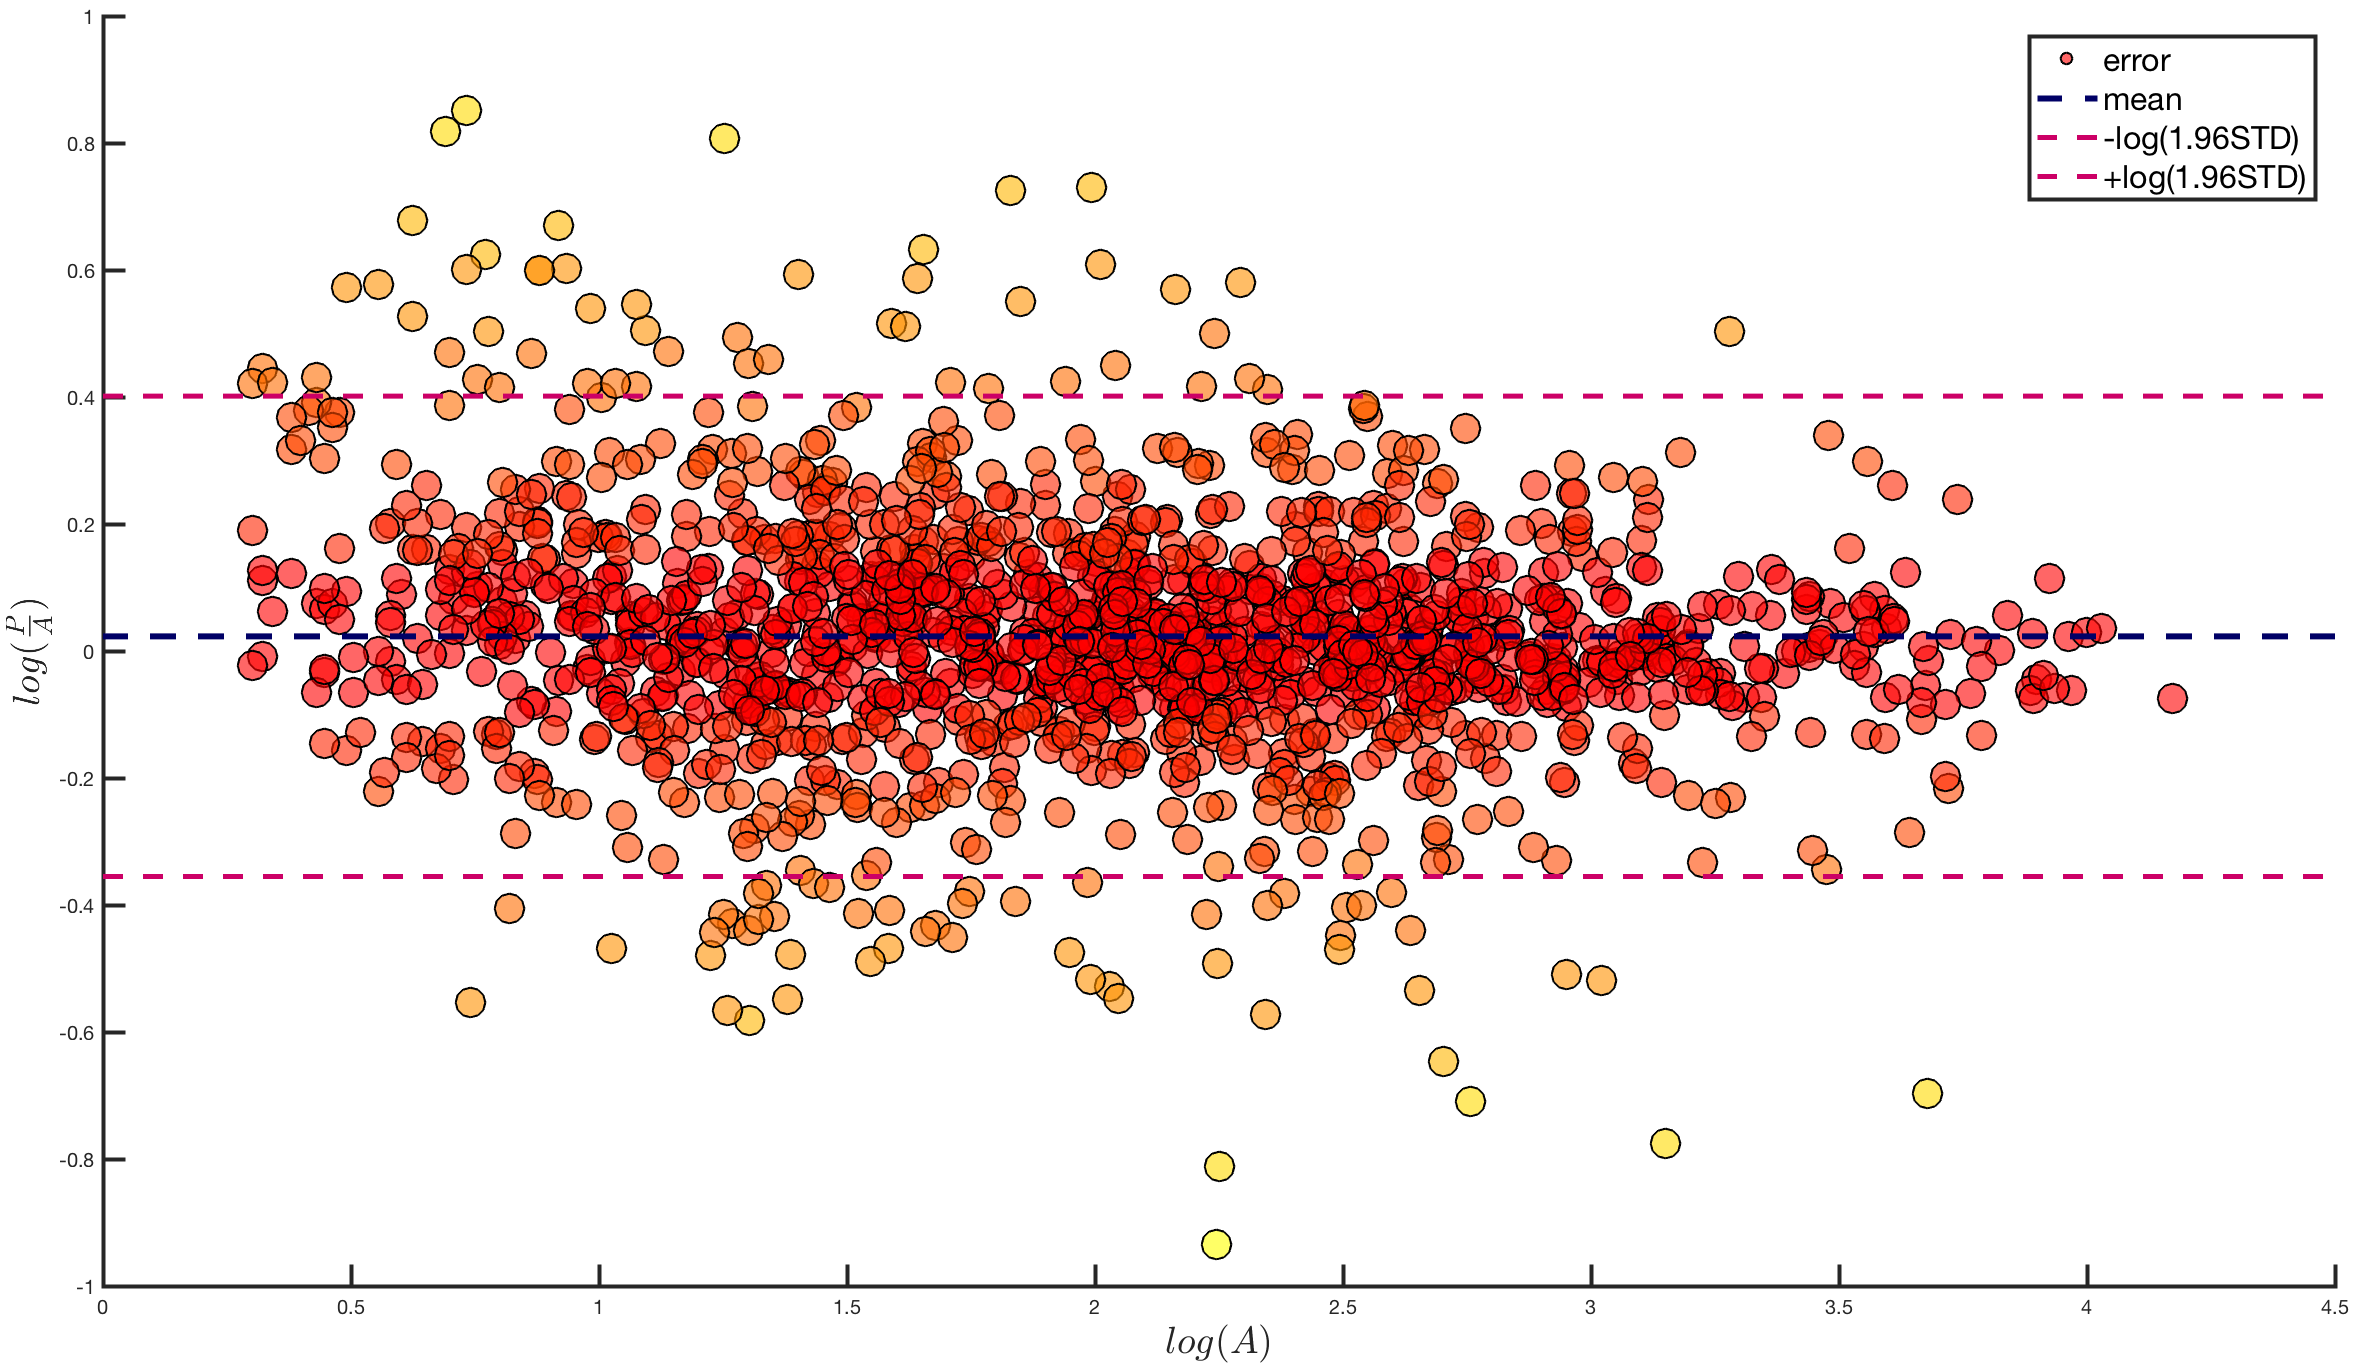
\includegraphics[width=.8\columnwidth]{figs/aguil13.png} \\
      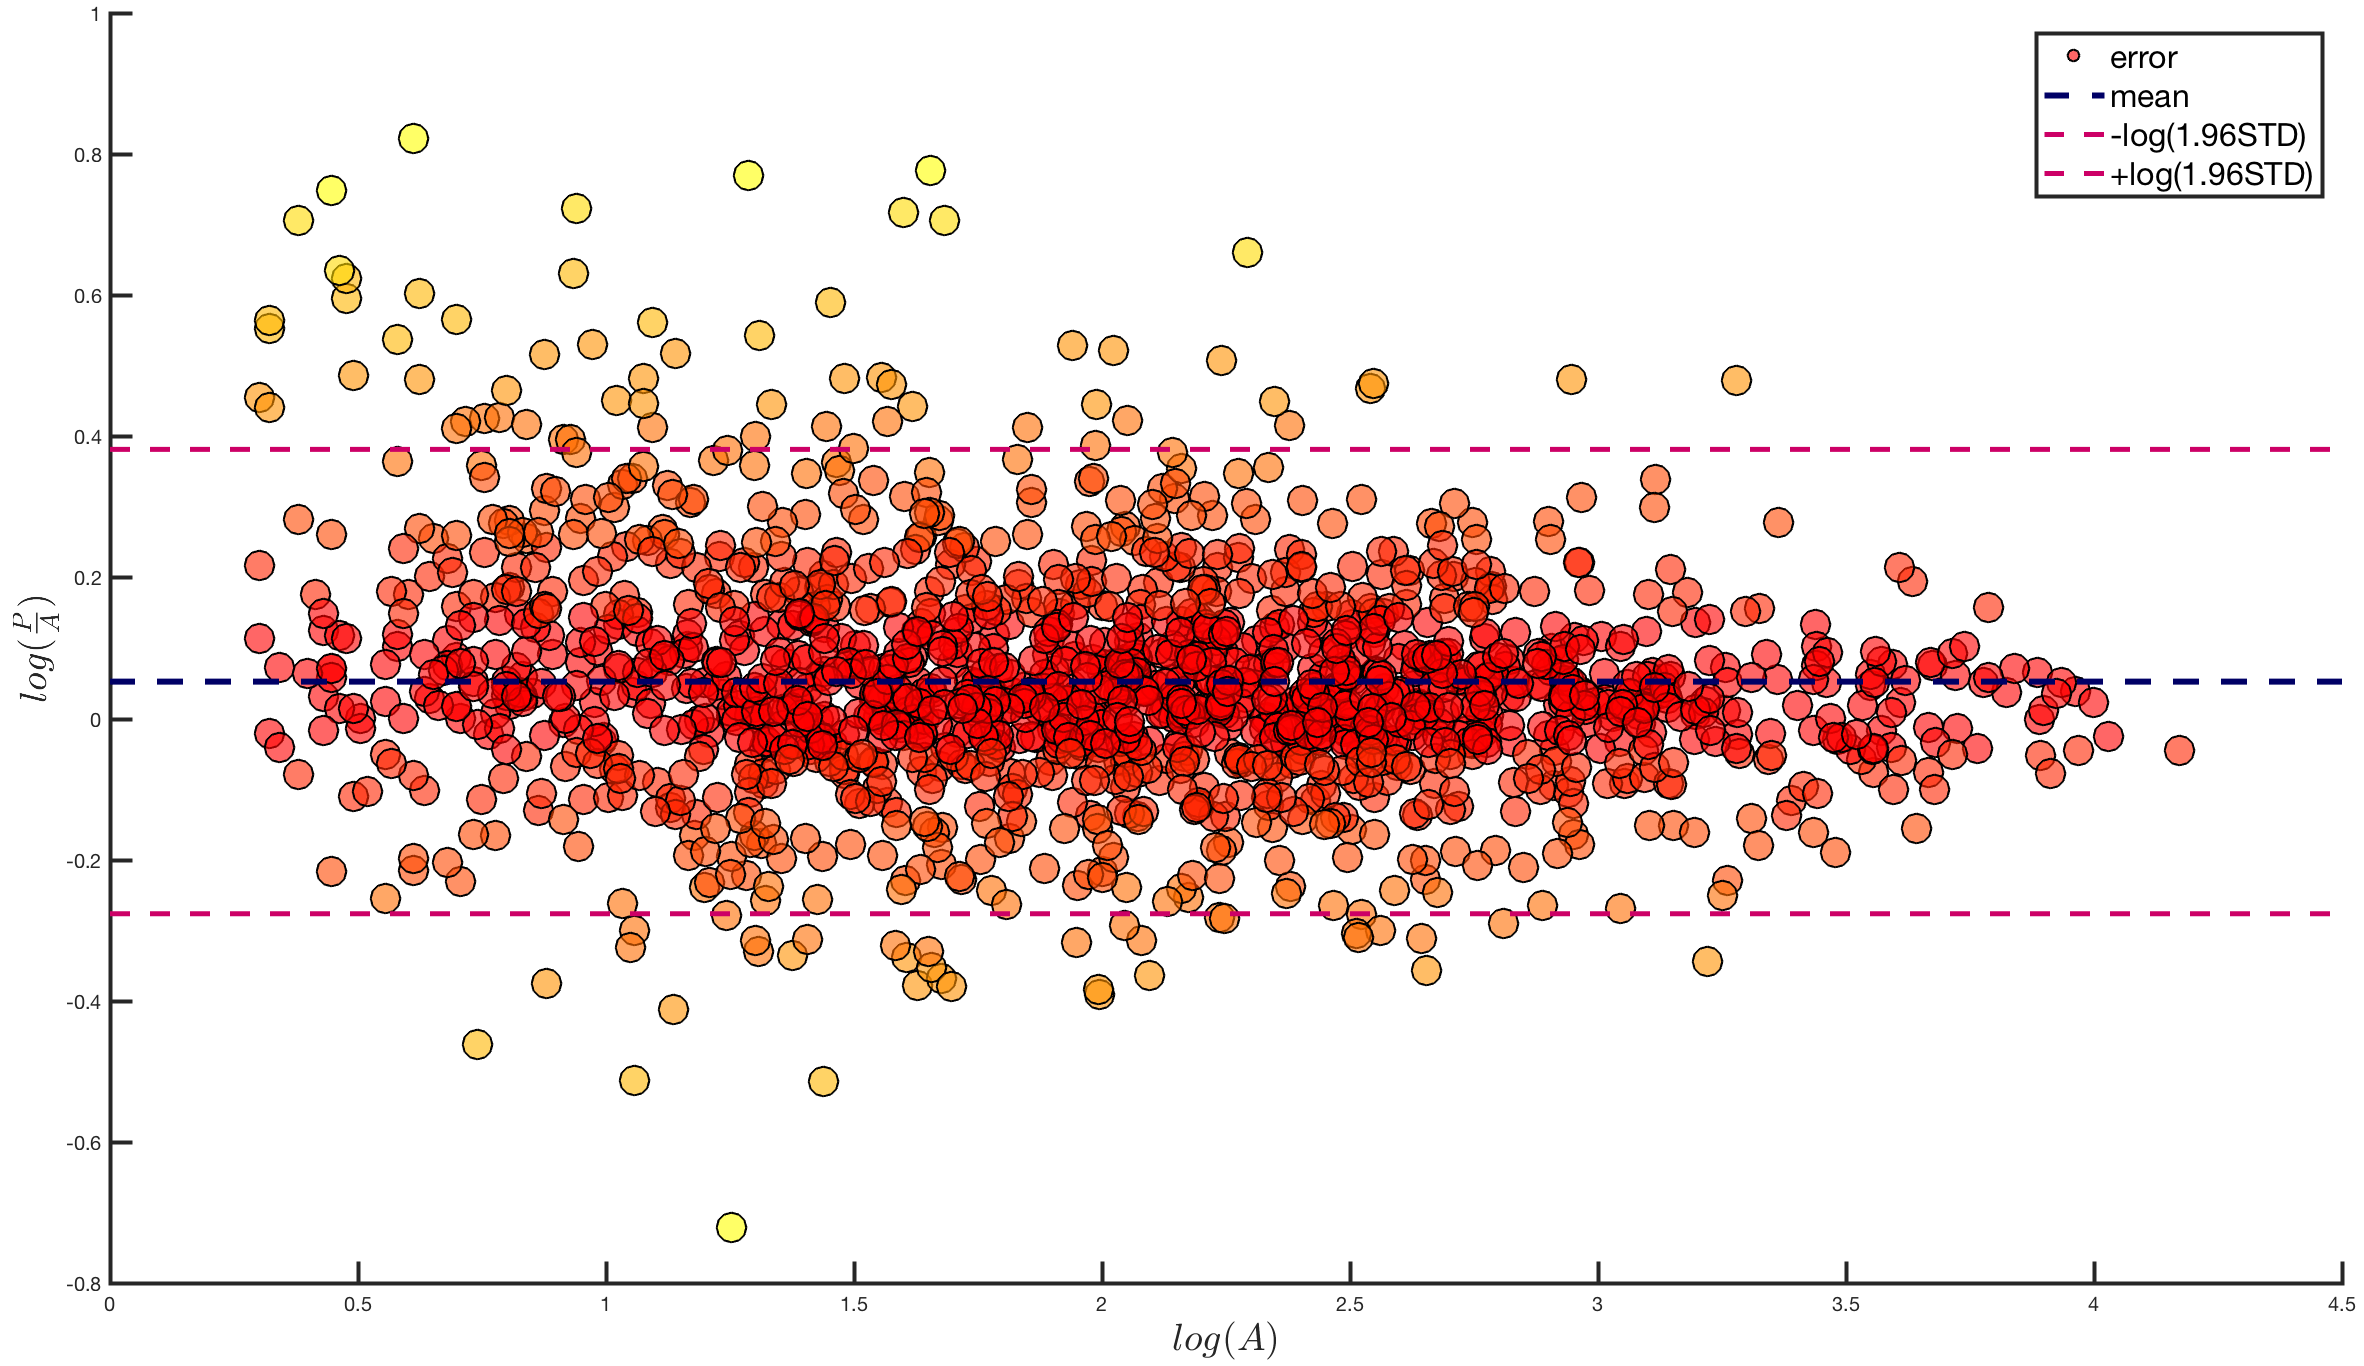
\includegraphics[width=.8\columnwidth]{figs/aguil12.png} \\
 \end{tabular}
      \caption{Bland-Altman difference plot in logarithmic scale for medium-large stores from a European country for category Food 2. Top row shows the forecast produced by our method whereas the bottom row shows the benchmark. The forecast error is scale-free and mostly contained within the 2$\sigma$ bands.}
\label{fig:resultsUKBlandAltman}
\end{figure}

% Bland-Altman discussion
It is also interesting to discuss the distribution of the prediction errors. Graphical approaches such as the Bland-Altman differences plot \cite{bland1986statistical}, which scatters the residuals of the prediction against the actual value, allow to easily identify model anomalies such as bias, variance and heteroscedasticity. Due to the diversity of this dataset, the sales range in orders of magnitude and the linear scale Bland-Altman plot skews towards the high sales values, so we use a natural logarithm scale. Inspecting Figure \ref{fig:resultsUKBlandAltman} shows that the forecast error from our method is decently independent of the volume and close to homoscedasticity, being the majority of the residuals contained within 2 standard deviations. This figure also shows in the bottom row the plot for the benchmark. Both charts show overpredicted values for some slow seller products, indicating promotions that have underperformed compared to the historical records.

Finally, the third dataset contains the promotions of 3774 products in an Asian country with all types of stores. This market is largely more volatile than the European ones, and influenced by external factors that are either not captured in the dataset or unable to be explained or accounted for. That causes the forecast from the three techniques to be not as accurate as in the other datasets. In this example, the overall performance of our method is better than the other two techniques. There are two categories, non-food-2 and fresh-2, where the benchmark is just above, and in the category packed-food-3 our method is remarkably better. Table \ref{tab:GlobalResults} shows the drop in accuracy for this third dataset.

%-------------------------------------------------%
\section{Revisiting the Method: Corrections and Extensions} \label{sect:Revision}
%-------------------------------------------------%

\myblue{A retrospective review of the method, conducted with the benefit of
several years of developments in the field, identified a number of points where
the formulation can be corrected, sharpened, or extended. This section presents
those revisions. We first situate the method within the metric-learning
literature, then correct two issues in the estimator and in the selection of the
number of neighbours, extend the point forecast into a calibrated predictive
distribution, describe three alternative similarity engines, and finally propose
an evaluation that makes the interpretability claim falsifiable. All revisions
are accompanied by a reference implementation and reproducible experiments.}

\subsection{Relationship to metric learning} \label{subSect:metricLearning}

\myblue{The procedure of Section \ref{sect:Model} can be read as learning a
non-negative \emph{diagonal Mahalanobis metric}. The weighted average of
Eq.\eqref{eqn:eqminus1} with the inverse-distance weights of
Eq.\eqref{eqn:eq8} is precisely a Nadaraya--Watson kernel regressor whose kernel
is parametrised by the feature-importance vector $\mathbf{v}$. Choosing
$\mathbf{v}$ to minimise the forecast error, as posed in Eq.\eqref{eqn:eq3}, is
the objective of Metric Learning for Kernel Regression (MLKR)
\cite{weinberger2007metric}, which learns a Mahalanobis metric by minimising the
leave-one-out regression error and is solved by gradient descent. The
contribution of our method is therefore not the objective itself but the
\emph{tractable surrogate} used to solve it: rather than optimising
Eq.\eqref{eqn:eq3} directly, we impose the identity of Eq.\eqref{eqn:eq5} and
recover $\mathbf{v}$ from the linear NNLS problem of Eq.\eqref{eqn:nnlsMatrix}.
This connection clarifies both the method's behaviour and its limitations: the
adaptive-neighbourhood view also underlies the interpretation of random forests
as nearest-neighbour estimators \cite{lin2006random}, which we exploit in
Section \ref{subSect:engines}.}

\subsection{Correcting the estimator and the selection of $k$} \label{subSect:corrections}

\myblue{\emph{Selection of the number of neighbours.} Equation
\eqref{eqn:eq_kNN} selects, for each validation promotion, the number of
neighbours minimising the relative absolute error, and the global value is then
averaged across the validation set. Care must be taken in the aggregate
criterion: minimising the absolute value of the \emph{mean signed} error across
the validation set,}
\begin{equation}
k_\mathrm{bias} = \underset{k}{\arg\min} \left| \frac{1}{P}\sum_{p=1}^{P} \left( \hat{y}_p^{(k)} - y_p \right) \right|,
\label{eqn:kSelBias}
\end{equation}
\myblue{rewards configurations in which positive and negative errors cancel
rather than configurations that are individually accurate, and it
systematically favours larger neighbourhoods. The criterion should instead be
the \emph{mean absolute} error,}
\begin{equation}
k^\star = \underset{k}{\arg\min} \; \frac{1}{P}\sum_{p=1}^{P} \left| \hat{y}_p^{(k)} - y_p \right|.
\label{eqn:kSelCorrect}
\end{equation}
\myblue{The same argument applies jointly to the kernel bandwidth introduced
below. As reported in Section \ref{subSect:revisedResults}, this single change
accounts for a reduction of roughly $9$--$11\%$ in mean absolute error on the
surrogate model of Section \ref{subSect:muticol}.}

\myblue{\emph{Noise floor.} Expanding the squared response difference of
Eq.\eqref{eqn:eq5} for an additive-error model $y = \boldsymbol{\beta}^\top
\mathbf{x} + \varepsilon$ shows that $\mathbb{E}\!\left[(y_k - y_i)^2\right]$
contains an irreducible term $2\sigma_\varepsilon^2$ for every pair, regardless
of feature proximity. Since the NNLS system of Eq.\eqref{eqn:nnlsMatrix} has no
constant term, this offset is absorbed into $\mathbf{v}$ and biases the learned
importances. Augmenting the design with a constant column,}
\begin{equation}
\begin{aligned}
\{\hat{\mathbf{v}}, \hat{c}\} =~ & \underset{\mathbf{v} \geq \mathbf{0},\, c \geq 0}{\arg\min}
& \norm{ \left[\mathbf{M} \;\; \mathbf{1}\right] \begin{bmatrix} \mathbf{v} \\ c \end{bmatrix} - \mathbf{e} }_2^2 + \lambda^2 \norm{ \mathbf{v} }_2^2 ,
\end{aligned}
\label{eqn:nnlsIntercept}
\end{equation}
\myblue{lets the intercept $\hat{c}$ estimate the noise floor $2\sigma_\varepsilon^2$
(a useful diagnostic in itself) while leaving $\mathbf{v}$ to capture only the
feature-dependent structure.}

\myblue{\emph{Scale of the response.} The loss of Eq.\eqref{eqn:nnlsMatrix} is a
squared error on \emph{squared} response differences, so the response enters at
the fourth power. For the heavy-tailed promotional sales of
Figure \ref{fig:fakeProduct}, a handful of extreme pairs then dominate the
solution. When the multiplicative component of the noise dominates, learning the
metric on $\log(1+y)$ removes this sensitivity and aligns the training loss with
the NRMSLE used in Section \ref{subSect:TescoData}; when the additive component
dominates, the original scale is preferable. As the appropriate scale is a
property of the data, our implementation fits both and retains the one with the
lower validation error.}

\myblue{Finally, we note that Eq.\eqref{eqn:eq5} asserts $\mathbf{m}^i\mathbf{v}
\approx 0$ whenever $y_i \approx y_k$, even for promotions that are similar in
response only by coincidence. Such pairs drive the importances of genuinely
relevant features towards zero. The MLKR formulation of
Section \ref{subSect:metricLearning} avoids this, as it never imposes the
bidirectional identity; an inexpensive alternative within the present framework
is to down-weight pairs with small $|y_k - y_i|$, since the implication
``far in response $\Rightarrow$ far in features'' is sound while its converse is
not.}

\subsection{From point forecasts to calibrated distributions} \label{subSect:probabilistic}

\myblue{Inventory decisions for promotions are newsvendor problems: the
quantity to order is a quantile of the demand distribution whose level is set by
the ratio of understocking to overstocking costs, which for perishable goods are
strongly asymmetric. A point forecast does not answer this question, yet the
method already computes everything required to do so. The $k$ retrieved
neighbours, with normalised weights $\tilde{w}_i = w_i / \sum_{j} w_j$ and
responses $y_i$, define a weighted empirical predictive distribution,}
\begin{equation}
\hat{F}(t \mid \mathbf{x}) = \sum_{i=1}^{k} \tilde{w}_i \, \mathbb{I}\!\left[y_i \leq t\right],
\label{eqn:predCDF}
\end{equation}
\myblue{whose generalised inverse $\hat{F}^{-1}(\tau \mid \mathbf{x})$ yields the
$\tau$-quantile required by the newsvendor rule, at no additional computational
cost. To equip these quantiles with finite-sample guarantees we apply
conformalised quantile regression \cite{romano2019cqr}, reusing the validation
set $\{(\mathbf{x}_p, y_p)\}_{p=1}^{P}$ already maintained for the selection of
$k$ as a calibration set. For a target miscoverage $\alpha$, define the
conformity scores}
\begin{equation}
E_p = \max\!\left\{ \hat{F}^{-1}(\tfrac{\alpha}{2}\mid \mathbf{x}_p) - y_p,\; y_p - \hat{F}^{-1}(1-\tfrac{\alpha}{2}\mid \mathbf{x}_p) \right\},
\label{eqn:cqrScore}
\end{equation}
\myblue{and let $Q_{1-\alpha}$ be the $\lceil (P+1)(1-\alpha)\rceil / P$ empirical
quantile of $\{E_p\}$. The interval}
\begin{equation}
\mathcal{C}(\mathbf{x}) = \left[\, \hat{F}^{-1}(\tfrac{\alpha}{2}\mid \mathbf{x}) - Q_{1-\alpha},\;\; \hat{F}^{-1}(1-\tfrac{\alpha}{2}\mid \mathbf{x}) + Q_{1-\alpha} \,\right]
\label{eqn:cqrInterval}
\end{equation}
\myblue{then satisfies $\Pr\!\left[y \in \mathcal{C}(\mathbf{x})\right] \geq
1-\alpha$ under exchangeability, distribution-free
\cite{lei2018distribution}. The interpretability of the method is preserved and
arguably improved: instead of a single number, the forecaster is shown the range
of outcomes of the similar historical promotions and the order quantity that
attains a target service level.}

\subsection{Alternative similarity engines} \label{subSect:engines}

\myblue{The value of the method to its users lies in the \emph{interface} --- a
forecast expressed as an editable, weighted set of comparable past promotions
--- rather than in the particular way the similarity is computed. This
observation admits several drop-in replacements for the engine that preserve the
interface while addressing the limitations of the diagonal NNLS metric.}

\myblue{\emph{Gradient-based MLKR.} The objective of Eq.\eqref{eqn:eq3} can be
optimised directly by gradient descent over a non-negative diagonal metric. The
computational objection raised in Section \ref{sect:Model} no longer applies at
the per-SKU scale of tens to a few hundred promotions, where convergence is
attained in milliseconds, and the resulting metric does not suffer from the
bidirectional-identity artefact of Section \ref{subSect:corrections}.}

\myblue{\emph{Random-forest proximities.} Interpreting a regression forest as an
adaptive nearest-neighbour rule \cite{lin2006random}, the fraction of trees in
which two promotions fall in the same leaf provides a similarity that captures
feature interactions and is insensitive to monotone feature transformations,
while the forecast remains a weighted average of retrieved promotions.}

\myblue{\emph{Global retrieval-augmented forecasting.} The per-SKU design treats
each product independently, which discards cross-product structure and, more
critically, leaves no model at all for a newly introduced product. The evidence
accumulated since the M5 competition \cite{makridakis2022m5} indicates that
models trained jointly across series are advantageous on retail data precisely
because of such cross-learning. We therefore train a single model across all
products, using product descriptors as additional features, and take its
internal representation $\boldsymbol{\phi}(\mathbf{x})$ as an embedding in which
neighbours are retrieved,}
\begin{equation}
d^2(\mathbf{x}, \mathbf{x}_i) = \norm{ \boldsymbol{\phi}(\mathbf{x}) - \boldsymbol{\phi}(\mathbf{x}_i) }_2^2 ,
\label{eqn:embedDist}
\end{equation}
\myblue{after which the predictive distribution and conformal calibration of
Section \ref{subSect:probabilistic} apply unchanged. Prior-fitted networks for
tabular data \cite{hollmann2025tabular} are a natural choice of embedder, as the
small per-product contexts are well within their operating regime and require no
training. As reported below, this engine is complementary rather than
universally superior: it is outperformed by the per-SKU method when products
have ample independent history, and it is decisively better in the cold-start
regime that the original method cannot address at all.}

\subsection{Making interpretability testable} \label{subSect:loop}

\myblue{The paper argues that an editable forecast is operationally valuable
because forecasters can correct it, but it evaluates only automatic accuracy.
This claim can be made falsifiable. Consider a forecaster of skill $s \in
[0,1]$ who observes, through a channel of fidelity $s$, whether each retrieved
promotion is representative of the case at hand. Two interaction modes can then
be compared: an \emph{accept/reject} mode, in which the only available action is
to veto the forecast and revert to a baseline --- all that a non-interpretable
model affords --- and an \emph{edit} mode, in which the forecaster down-weights
the promotions judged unrepresentative and the forecast is recomputed. The
operational worth of interpretability is the accuracy gap between the two modes.
In a controlled simulation (Section \ref{subSect:revisedResults}) this gap is
positive at every skill level and grows with skill, providing quantitative
support for the editability argument; a study with human forecasters on the
real datasets remains the natural next step.}

\subsection{Revised experimental results} \label{subSect:revisedResults}

\myblue{Table \ref{tab:revisedAblation} reports an ablation on the surrogate
model of Section \ref{subSect:muticol}, averaged over five realisations. The
legacy configuration reproduces the originally published figures (e.g.
$w20p\approx55$ on the ideal case), validating the setup. Correcting the
selection of $k$ alone removes a substantial fraction of the error; the
corrected estimator (intercept of Eq.\eqref{eqn:nnlsIntercept}, validated
response scale, Gaussian kernel) improves it further, and the gradient-based
MLKR engine is best overall, most clearly under collinearity --- consistent with
the analysis of Section \ref{subSect:corrections}. The conformalised intervals
of Eq.\eqref{eqn:cqrInterval} attain empirical coverage of $0.78$--$0.82$ at the
nominal $80\%$ level across all scenarios.}

\begin{table}[t]
\centering
\resizebox{\columnwidth}{!}{
\begin{tabular}{lccc}
\toprule
Variant & MAE & $w20p$ (\%) & $out50p$ (\%) \\
\midrule
Legacy (original) & 1227 & 54.3 & 12.5 \\
Legacy + corrected $k$ (Eq.\eqref{eqn:kSelCorrect}) & 1110 & 59.0 & 9.0 \\
Uniform-weight $k$NN (ablation) & 1209 & 52.3 & 11.8 \\
Corrected estimator & 1080 & 58.8 & 8.1 \\
Diagonal MLKR & 1061 & 60.6 & 7.7 \\
Random-forest proximities & 1063 & 62.2 & 8.5 \\
\bottomrule
\end{tabular}
}
\caption{\myblue{Ablation on the surrogate model of Section
\ref{subSect:muticol} (mean over the ideal, collinearity and endogeneity
scenarios, five realisations). Correcting the selection of $k$ alone removes a
large fraction of the error, and the metric-learning engines improve on it
further. The uniform-weight row isolates the contribution of metric learning.}}
\label{tab:revisedAblation}
\end{table}

\myblue{Two further experiments evaluate the extensions of
Sections \ref{subSect:engines} and \ref{subSect:loop}. For cross-SKU
retrieval, the global engine is compared with the per-SKU method across three
regimes (ten realisations each): with ample per-product history and no shared
structure the per-SKU method is far superior (the global embedding adds only
variance); with short histories sharing structure through descriptors the two
are comparable; and for brand-new products with no history --- the failure mode
acknowledged in Section \ref{sect:Conclusion} --- the per-SKU method can only
return a global average ($\mathrm{MAE}\approx412$), whereas the descriptor-based
global engine reduces the error by about two thirds ($\mathrm{MAE}\approx136$).
The retrieval engine should therefore be deployed alongside, not in place of,
the per-SKU method, to cover cold-start cases. For the forecaster-in-the-loop
simulation, the editing mode improves on accept/reject at every skill level; at
full skill it reduces mean absolute error by about $21\%$ relative to the
automatic forecast and more than halves the volume forecast with an error above
$50\%$, while the accept/reject mode never improves on the automatic forecast.}

%-------------------------------------------------%
\section{Conclusion} \label{sect:Conclusion}
%-------------------------------------------------%

The accurate prediction of promotional sales is of paramount importance for customers, retailers, producers and suppliers. Amongst others, one of the benefits that the authors would like to highlight is waste reduction. This paper presented a new forecasting method inspired in the know-how of the business analysts, or forecasters, that tackle the problem of sales forecasting on a daily basis. That motivated us to work on a kNN method that produces explainable and easy to modify predictions. Also, we wanted to couple feature selection and prediction, which we accomplished through a cost function that is minimised with a NNLS solver. Our method is founded on online learning, so the predictions are calculated with the latest data available, thus avoiding to retrain the model. Also, the forecast is generated at SKU level meaning that the data always fits in memory. Beyond the basic formulation of our model, we have shown how to extend it by combining single learners and weak forecasters to improve prediction accuracy and can be run in a parallel. To validate our method, we have conducted several experiments. On surrogate models, we have demonstrated that the method is able to find the features related to sales, even in an scenario where the sales are driven by a variable that is present very little times, our method is able to identify that key variable. On real-market datasets, we have demonstrated that we can significantly improve the accuracy of the forecast by improving the benchmark in many diverse categories and geographical locations. We have also compared the method against a 100 decision trees model trained on the same data, an the results prove that our method is much more suitable for promotional forecasting applications. In terms of interpretability, the method feedbacks both the most prominent features and the weights of the promotions used to calculate the forecast. As many promotions, especially the cost-sensitive ones, get reviewed and adjusted by forecasters, they can easily control the historical promotions that contribute to the forecast by modifying the weights. Known limitations of the model arise in the following scenarios. When the values of the observed historical KPIs are far from the ones to be predicted, the model is unable to produce accurate forecast. For example, consider a product that is trendy at the time of forecast but the historical sales do not reflect that (or viceversa). Another source of inaccuracy is found when the predictors do not contain meaningful information about the KPI, so that the feature selection process assigns similar importance values. Future work will concentrate on exploring different distance measures to calculate the feature importance weights, a bit less restrictive than Eq.~ \ref{eqn:eq4}; \myblue{several such directions, together with corrections to the present formulation and a probabilistic extension of the forecast, are developed in Section \ref{sect:Revision}.} Fortunately for us, the categorical data in our datasets present low cardinality. However, in the case of large cardinality we recommend to apply some dimensionality reduction such as the popular Entity Embeddings \cite{Guo2016emb}. As a final note in the Appendix, we outline how to deploy our method in a production environment running on a cloud provider.

\appendices

\section{Appendices}
\subsection{Forecast metrics} \label{app:ForecastErrors}

Table~\ref{tab:FrcErrors} summarises the calculation of the forecast metrics used in this paper.

\begin{table*}[t] 
\centering
\resizebox{\textwidth}{!}{
\begin{tabular}{p{6cm}cc}
\hline
Metric & Short name & Equation \\
\hline
%Forecast Error  &      frcErr      &      $\frac{\sum_{i=1}^{N} | y_i-\hat{y}_i |}{\sum_{i=1}^{N} y_i}$   \\
%Forecast Error  &      frcErr      &      $\frac{1}{\sum_{i=1}^{N} y_i} \sum_{i=1}^{N} | y_i-\hat{y}_i |$   \\
Forecast Error  &      frcErr      &      $ \sum_{i=1}^{N} | y_i-\hat{y}_i | / \sum_{i=1}^{N} y_i$   \\
%Forecast Bias & frcBias & $\frac{\sum_{i=1}^{N} y_i-\hat{y}_i}{\sum_{i=1}^{N} \hat{y}_i}$ \\
Forecast Bias & frcBias & $\sum_{i=1}^{N} (y_i-\hat{y}_i) / \sum_{i=1}^{N} \hat{y}_i$ \\
%Forecast Accuracy & frcAcc & $1 - \frac{\sum_{i=1}^{N} y_i-\hat{y}_i}{\sum_{i=1}^{N} \hat{y}_i}$ \\
Forecast Accuracy & frcAcc & 1 - frcBias \\
Forecast Mean Absolute Error   &    frcMAE & $\frac{1}{N} \sum_{i=1}^{N} | y_i-\hat{y}_i |$ \\

Root Mean Squared Error &  RMSE  &  $\sqrt{\mathbb{E} \left[ ( \mathbf{y}-\hat{\mathbf{y}} )^2 \right]}$\\
Mean Absolute Percentage Error & MAPE & $\frac{100}{N}\sum_{i=1}^{N}\left| \frac{y_{i}-\hat{y}_{i}}{y_{i}} \right|$ \\
Normalised Root Mean Squared Logarithmic Error & NRMSLE & $\sqrt{\frac{1}{N}\sum_{i=1}^{N} \ln \left( \frac{1+\hat{y}_{i}}{1+ y_{i}} \right)^2}$ \\

\hline
\end{tabular}
}
\caption{Summary of the forecast measures used along the paper.} 
\label{tab:FrcErrors}
\end{table*}


\subsection{Forecast as a (micro) Service} \label{app:FrcAsService}

Data science teams traditionally operate as autonomous teams, developing and deploying independently from other teams. The method presented in this paper is no exception to this rule and it has been architectured as a micro-service to be called from the forecaster's system, usually a web application.

We make use of several Open Source solutions for this to happen. The first one is the coding language, where we have chosen Python 3~\cite{Python} for many obvious reasons. To attend forecast requests, formed as JSON~\cite{JSON} representations, we have chosen Flask~\cite{Flask}, as it is a friendly and lightweight Python-based web micro-framework. Docker~\cite{Docker} containers are a great solution for deploying in the majority of cloud providers and in our case, the configuration file (Dockerfile) to build the container is decently simple.

One consideration in our deployment is to avoid database or storage dependencies to improve modularity. As the number of historical promotions is relatively small and so is the number of features (as opposed to Big Data), the REST request contains both the data to forecast for, but also the historical records. The response of our micro-service is composed of the forecast but also the weights assigned to the relevant historical promotions.

The schema \ref{app:FrcAsService} illustrates this solution that we have successfully deployed and tested.

\begin{figure*}[t]
  \centering 
  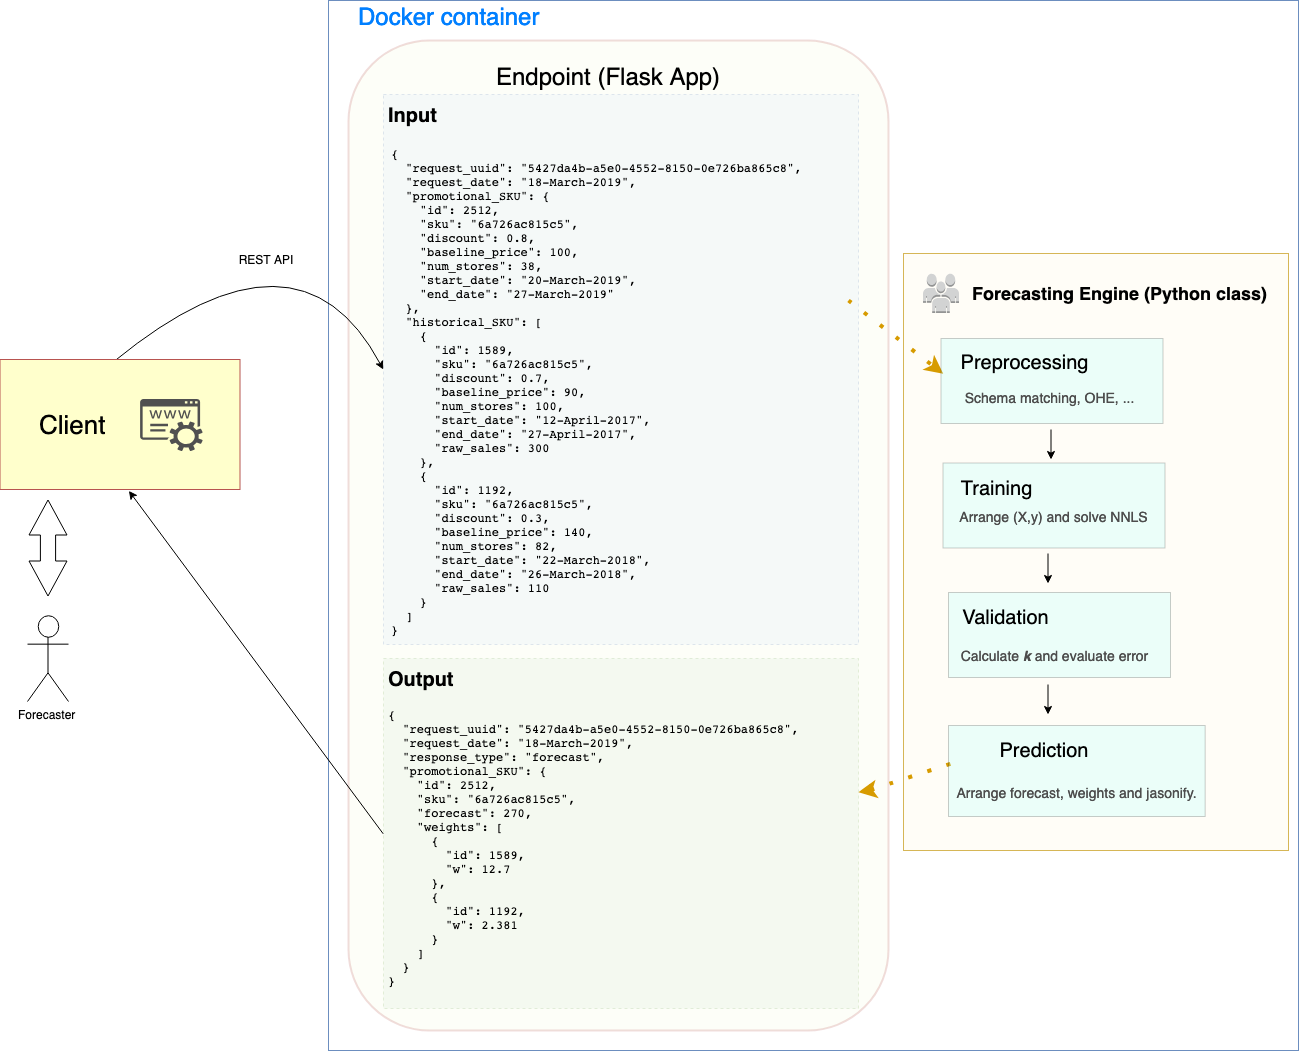
\includegraphics[width=\textwidth]{figs/aguil14.png} 
  \caption{Running the forecast as a service. Open Source software allows to easily productionalise applications such as the forecasting method described in this paper. The main engine is a Python class that is served with Flask running in a Docker container, which attends requests where the payload is JSON coded.}
  \label{fig:FrcAsAService}
\end{figure*}


%\section*{Acknowledgment}
%This work was partly supported by Research Grants FINALE, and KERMES (TEC2016-75161-C2-1-R, and 
%TEC2016-81900-REDT/AEI) from Spanish Government.


\begin{thebibliography}{00}

\bibitem{gomez2007empirical}
M.~I. G{\'o}mez, V.~R. Rao, E.~W. McLaughlin, Empirical analysis of budget and
  allocation of trade promotions in the {US} supermarket industry, Journal of
  Marketing Research 44~(3) (2007) 410--424.

\bibitem{ailawadi2006promotion}
K.~L. Ailawadi, B.~A. Harlam, J.~Cesar, D.~Trounce, Promotion profitability for
  a retailer: the role of promotion, brand, category, and store
  characteristics, Journal of Marketing Research 43~(4) (2006) 518--535.

\bibitem{natter2007practice}
M.~Natter, T.~Reutterer, A.~Mild, A.~Taudes, Practice prize report—an
  assortmentwide decision-support system for dynamic pricing and promotion
  planning in {DIY} retailing, Marketing Science 26~(4) (2007) 576--583.

\bibitem{blattberg1990sales}
R.~C. Blattberg, S.~A. Neslin, Sales promotion: Concepts, methods, and
  strategies, Prentice Hall Englewood Cliffs, NJ, 1990.

\bibitem{blattberg1995promotions}
R.~C. Blattberg, R.~Briesch, E.~J. Fox, How promotions work, Marketing Science
  14~(3\_supplement) (1995) G122--G132.

\bibitem{fildes2016use}
R.~Fildes, P.~Goodwin, D.~Onkal, Use and misuse of information in supply chain
  forecasting of promotion events, Workingpaper, Department of Management
  Science, Lancaster University (10 2016).

\bibitem{alamdar2018pricing}
S.~F. Alamdar, M.~Rabbani, J.~Heydari, Pricing, collection, and effort
  decisions with coordination contracts in a fuzzy, three-level closed-loop
  supply chain, Expert Systems with Applications 104 (2018) 261--276.

\bibitem{ma2017retail}
S.~Ma, R.~Fildes, A retail store sku promotions optimization model for category
  multi-period profit maximization, European Journal of Operational Research
  260~(2) (2017) 680--692.

\bibitem{van2016analysis}
K.~Van~Donselaar, J.~Peters, A.~De~Jong, R.~Broekmeulen, Analysis and
  forecasting of demand during promotions for perishable items, International
  Journal of Production Economics 172 (2016) 65--75.

\bibitem{di2016application}
G.~Di~Pillo, V.~Latorre, S.~Lucidi, E.~Procacci, An application of support
  vector machines to sales forecasting under promotions, 4OR (Quarterly Journal
  of Operations Research) 14~(3) (2016) 309--325.

\bibitem{ramanathan2011identifying}
U.~Ramanathan, L.~Muyldermans, Identifying the underlying structure of demand
  during promotions: A structural equation modelling approach, Expert Systems
  with Applications 38~(5) (2011) 5544--5552.

\bibitem{ali2009sku}
{\"O}.~G. Ali, S.~Say{\i}n, T.~Van~Woensel, J.~Fransoo, {SKU} demand
  forecasting in the presence of promotions, Expert Systems with Applications
  36~(10) (2009) 12340--12348.

\bibitem{louis2013analysts}
H.~Louis, A.~X. Sun, O.~Urcan, Do analysts sacrifice forecast accuracy for
  informativeness?, Management Science 59~(7) (2013) 1688--1708.

\bibitem{LIU2011fast}
Y.~Liu, F.~Sun, A fast differential evolution algorithm using k-nearest
  neighbour predictor, Expert Systems with Applications 38~(4) (2011) 4254 --
  4258.

\bibitem{CHEN2017feature}
Y.~Chen, Y.~Hao, A feature weighted support vector machine and k-nearest
  neighbor algorithm for stock market indices prediction, Expert Systems with
  Applications 80 (2017) 340 -- 355.

\bibitem{martinez2018dealing}
F.~Mart{\'\i}nez, M.~P. Fr{\'\i}as, M.~D. P{\'e}rez-Godoy, A.~J. Rivera,
  Dealing with seasonality by narrowing the training set in time series
  forecasting with knn, Expert Systems with Applications 103 (2018) 38--48.

\bibitem{shin2010firms}
T.~T. Shin~H, Do firms invest in forecasting efficiently? the effect of
  competition on demand forecast investments and supply chain coordination,
  Operations Research 58~(6) (2010) 1592--1610.

\bibitem{Shugan2004end}
S.~M. Shugan, Endogeneity in marketing decision models (2004).

\bibitem{bland1986statistical}
J.~M. Bland, D.~Altman, Statistical methods for assessing agreement between two
  methods of clinical measurement, The Lancet 327~(8476) (1986) 307--310.

\bibitem{Guo2016emb}
C.~Guo, F.~Berkhahn, Entity embeddings of categorical variables, arXiv preprint
  arXiv:1604.06737.

\bibitem{Python}
Python website, \url{https://www.python.org/}, accessed: 2019-03-13.

\bibitem{Flask}
Flask website, \url{http://flask.pocoo.org/}, accessed: 2019-03-13.

\bibitem{Docker}
Docker website, \url{https://www.docker.com/}, accessed: 2019-03-13.

\bibitem{JSON}
Json website, \url{https://www.json.org/}, accessed: 2019-03-13.

\bibitem{weinberger2007metric}
K.~Q. Weinberger, G.~Tesauro, Metric learning for kernel regression, in:
  Proceedings of the Eleventh International Conference on Artificial
  Intelligence and Statistics (AISTATS), Vol.~2, 2007, pp. 612--619.

\bibitem{lin2006random}
Y.~Lin, Y.~Jeon, Random forests and adaptive nearest neighbors, Journal of the
  American Statistical Association 101~(474) (2006) 578--590.

\bibitem{makridakis2022m5}
S.~Makridakis, E.~Spiliotis, V.~Assimakopoulos, The {M5} competition:
  Background, organization, and implementation, International Journal of
  Forecasting 38~(4) (2022) 1325--1336.

\bibitem{romano2019cqr}
Y.~Romano, E.~Patterson, E.~Cand{\`e}s, Conformalized quantile regression, in:
  Advances in Neural Information Processing Systems (NeurIPS), Vol.~32, 2019,
  pp. 3543--3553.

\bibitem{lei2018distribution}
J.~Lei, M.~G'Sell, A.~Rinaldo, R.~J. Tibshirani, L.~Wasserman, Distribution-free
  predictive inference for regression, Journal of the American Statistical
  Association 113~(523) (2018) 1094--1111.

\bibitem{hollmann2025tabular}
N.~Hollmann, S.~M{\"u}ller, L.~Purucker, A.~Krishnakumar, M.~K{\"o}rfer, S.~B.
  Hoo, R.~T. Schirrmeister, F.~Hutter, Accurate predictions on small data with a
  tabular foundation model, Nature 637~(8045) (2025) 319--326.

\end{thebibliography}
%author, title, journal volume~(number) (year) pages.


\begin{IEEEbiography}[{
\includegraphics[width=1in,height=1.25in,clip,keepaspectratio]{figs/Carlos.png}}]{Carlos~Aguilar-Palacios} received a B.Sc and M.Sc in Telecommunications Engineering (2009) from Universidad Rey Juan Carlos and a M.Sc. in Physics and Mathematics (2011) from Universidad de Castilla-La Mancha. He is currently working towards the completion of his Ph.D. in Machine Learning at Universidad Rey Juan Carlos. 
\end{IEEEbiography}

% if you will not have a photo at all:
\begin{IEEEbiography}[{
\includegraphics[width=1in,height=1.25in,clip,keepaspectratio]{figs/Sergio.png}}]{Sergio~Muñoz-Romero} received a degree in Engineering (2009) and a Ph.D. in Machine Learning (2015) from Universidad Carlos III, Spain. His present research interest are centered in Machine Learning Algorithms and statistical learning theory, mainly dimensionality reduction ans feature selection methods.
\end{IEEEbiography}

% insert where needed to balance the two columns on the last page with
% biographies
%\newpage

\begin{IEEEbiography}[{
\includegraphics[width=1in,height=1.25in,clip,keepaspectratio]{figs/JL.png}}]{José~Luis~Rojo-Álvarez} Dr. Jose Luis Rojo Álvarez is a professor at the Department of Signal Theory and Communications in University Rey Carlos (Spain). He received a B.Sc. (1996) and the Ph.D. (2000) degrees on Telecommunication Engineering at University of Vigo and University Politécnica de Madrid, respectively. His research interests focus on statistical learning methods for signal and image processing, arrhythmia mechanisms, robust signal processing methods for cardiac repolarization, and Doppler image post-processing. He has (co)authored more than 120 international papers and has contributed to more than 160 conference proceedings.
\end{IEEEbiography}

\EOD

\end{document}
